\documentclass[UTF8,a4paper,12pt]{ctexart}

\usepackage{geometry}
\usepackage{amsmath,amssymb}
\usepackage{setspace}
\usepackage{indentfirst}
\usepackage{fancyhdr}
\usepackage{booktabs}
\usepackage{graphicx}
\graphicspath{{./figures/}}
\usepackage{float}
\usepackage{tikz}
\usepackage{array}
\usepackage{caption}
\setCJKmainfont[AutoFakeBold=3,AutoFakeSlant=0.2]{SimSun}
\setCJKsansfont[AutoFakeBold=3,AutoFakeSlant=0.2]{SimSun}
\setCJKmonofont[AutoFakeBold=3]{SimSun}
\usetikzlibrary{arrows.meta,positioning,shapes.geometric}
\captionsetup{font=small,labelfont=bf}

\newenvironment{pseudocode}
{\begin{tabular}{p{0.94\textwidth}}}
	{\end{tabular}}

% ==================== 页面格式 ====================
\geometry{
	left=2.5cm,
	right=2.5cm,
	top=2.5cm,
	bottom=2.5cm
}

% ==================== 页眉页脚 ====================
\pagestyle{fancy}
\fancyhf{}
\fancyfoot[C]{\zihao{-5}\thepage}
\renewcommand{\headrulewidth}{0pt}
\renewcommand{\footrulewidth}{0pt}

% ==================== 段落格式 ====================
\setlength{\parindent}{2em}
\setlength{\parskip}{0pt}

% ==================== 摘要重点词格式 ====================
\newcommand{\paperbold}{\CJKfontspec[AutoFakeBold=4]{SimSun}\bfseries}
\newcommand{\keypoint}[1]{{\paperbold #1}}
\newcommand{\modelsubpoint}[1]{\vspace{0.35em}\noindent{\paperbold #1}\par\vspace{0.12em}}

\begin{document}
	
	% ==================== 封面 ====================
	\thispagestyle{empty}
	\vspace*{7.2cm}
	{
		\songti\zihao{-2}
		\noindent 参赛题目：C 题
		
		\vspace{2.2cm}
		
		\noindent 参赛队伍校内编号：CQUPT-MMC-2026-00007
	}
	\newpage
	
	\setcounter{page}{1}
	
	% ==================== 题目 ====================
	{
		\centering
		{\paperbold\zihao{3} 基于三维装箱与集合覆盖的新能源汽车核心零部件\\[-0.05em]
			运输优化问题\par}
	}
	
	\vspace{0.25em}
	
	% ==================== 摘要标题 ====================
	{
		\centering
		{\paperbold\zihao{4} 摘\quad 要\par}
	}
	
	\vspace{0.05em}
	
	% ==================== 摘要正文 ====================
	{
		\fontsize{12pt}{13.8pt}\selectfont
		
		新能源汽车核心零部件运输具有\keypoint{货物规格差异显著、重量分布不均、装载姿态受限、承重安全要求高和多站点卸货顺序约束强}等特点。传统二维装载模型或独立车辆路径模型难以同时兼顾三维空间可行性、运输安全、卸货可达性和成本经济性。针对上述问题，本文构建了\keypoint{坐标级三维装载--多点配送协同优化模型}，并设计启发式求解、方案复核和一致性校验相结合的闭环框架，实现从货物坐标到车辆路径的系统优化。
		
		\keypoint{针对问题一}，本文以 HeavyEV 车厢为三维装载空间，综合考虑空间边界、货物不重叠、底部支撑、顶部承重、类别约束、车辆载重和 $x$ 方向重心约束，建立\keypoint{单车三维装载与重心控制模型}。目标函数采用字典序结构，以装入件数最大化为首要目标，并进一步比较装入体积、装入重量、重心偏移和安全裕度。求解时采用\keypoint{极点/角点候选位置生成、多排序策略、多随机种子扰动、合法姿态枚举和局部修复}方法搜索最优可行方案。计算结果表明，HeavyEV 最终装入\keypoint{$138$ 件}货物，体积利用率为\keypoint{$79.5228\%$}，载重利用率为\keypoint{$92.75\%$}，$x$ 方向重心为\keypoint{$356.2646\,\mathrm{cm}$}，经验证硬性违规数为\keypoint{$0$}。
		
		\keypoint{针对问题二}，本文在单车三维装载模型基础上引入 HeavyEV/LightEV 多车型选择、多站点路径和严格 LIFO 卸货阻挡约束，建立\keypoint{候选车次生成与集合覆盖选择模型}。首先枚举车型、站点组合和路径顺序，生成满足三维装载、载重、重心和严格 LIFO 检验的候选车次池；随后结合\keypoint{支配剪枝、集合覆盖选择、贪心兜底和车次合并}策略，以总运输成本最小为目标确定车辆组合与配送路线。最终方案使用\keypoint{$4$ 个车次}完成\keypoint{$203$ 件}货物配送，总运输成本为\keypoint{$3003.779500$ 元}，严格 LIFO 检查无违规，实现了装载坐标、车辆组合和路径方案的一体化呈现。
		
		\keypoint{针对问题三}，本文构造 8 个配送站点和 20 种规格货物的中大规模模拟数据集，进一步比较\keypoint{严格 LIFO、区块化装载和柔性 LIFO}三类策略。模型通过站点聚类、路线枚举、区块分配、倒箱统计、敏感性分析和 Pareto 比较，刻画车辆数量、运输成本、装载利用率和卸货复杂度之间的权衡关系。结果表明，严格 LIFO 策略需 $4$ 辆车，总成本为 $3575.798550$ 元；柔性/区块化策略使用\keypoint{$3$ 辆车}，总成本降至\keypoint{$2770.781835$ 元}，当前实例中倒箱件数和倒箱体积均为\keypoint{$0$}，体现出更好的车辆节约效果和成本优势。
		
		\keypoint{针对问题四}，本文构建了\keypoint{独立验证与一致性核验机制}，对装载越界、三维重叠、支撑与悬空、顶部承重、类别约束、车辆载重、车辆重心、严格 LIFO 阻挡、柔性倒箱、货物重复配送与遗漏等指标进行逐项检查，并形成结构化验证结论。该机制与求解模型共同构成“建模求解--坐标方案--独立验证--结果核验”的闭环。综上，本文方法能够在满足硬约束的前提下获得\keypoint{可验证、可复核的最优可行方案}，可为新能源汽车核心零部件的三维装载与多点配送组织提供决策支持。
		
		\vspace{0.18em}
		
		\indent{\paperbold 关键词：} 三维装箱；多点配送；LIFO 约束；集合覆盖；独立验证
		
	}
	
	
	% ==================== 正文标题格式：一级中文编号，二级以下阿拉伯编号 ====================
	\ctexset{
		section = {
			format = \paperbold\zihao{3}\centering,
			name = {,、},
			number = \chinese{section},
			aftername = {},
			beforeskip = 1.0em,
			afterskip = 0.8em
		},
		subsection = {
			format = \paperbold\zihao{4},
			name = {,},
			aftername = {\quad},
			beforeskip = 0.8em,
			afterskip = 0.4em
		},
		subsubsection = {
			format = \paperbold\zihao{-4},
			name = {,},
			aftername = {\quad},
			beforeskip = 0.6em,
			afterskip = 0.3em
		}
	}
	\renewcommand{\thesubsection}{\arabic{section}.\arabic{subsection}}
	\renewcommand{\thesubsubsection}{\arabic{section}.\arabic{subsection}.\arabic{subsubsection}}
	\setcounter{secnumdepth}{3}
	
	\newpage
	
	\section{问题重述}
	
	\subsection{问题背景}
	
	新能源汽车核心零部件运输受到车辆三维空间、货物物理属性、装卸顺序和运输成本的共同影响。题目给定 HeavyEV 与 LightEV 两种车型，以及动力电池、电控精密件、驱动电机、车身结构件和冷却液等多类货物。不同类别货物在摆放姿态、堆叠方式、承重限制、相邻关系和卸货顺序方面均有约束，因此本题是融合三维装箱、车辆选型、路径规划、重心控制和 LIFO 卸货约束的协同优化问题。
	
	\subsection{问题提出}
	
	问题一要求在 HeavyEV 单车内装载场景 A 货物。装载方案需满足车厢尺寸、车辆载重、货物不重叠、底部支撑、顶部承重、类别约束和 $x$ 方向重心约束，并在可行前提下尽可能提高装入件数、体积利用率和载重利用率，最终给出每件货物的三维坐标和摆放姿态。
	
	问题二要求完成场景 B 全部货物的多车型、多车辆、多站点配送。车辆可选择 HeavyEV 或 LightEV，每辆车可服务一个或多个站点，但必须严格满足 LIFO 卸货阻挡约束。目标是在所有货物恰好配送一次、所有车辆装载可行的前提下，使总运输成本尽可能低，并给出车辆组合、配送路线和车内三维装载坐标。
	
	问题三要求构造包含 8 个配送站点和 20 种规格货物的中大规模模拟数据集，并在该数据集上比较严格 LIFO、区块化装载和柔性 LIFO 三类策略。比较指标包括车辆数、运输成本、装载利用率、倒箱件数、倒箱体积及其敏感性结果，从而分析不同装卸策略在成本与操作复杂度之间的权衡。
	
	问题四要求构建独立验证机制，对前三问给出的装载坐标进行复核。验证内容包括空间越界、三维重叠、支撑与悬空、承重、类别约束、载重、重心、LIFO 阻挡、柔性倒箱统计以及货物遗漏和重复配送等。该机制用于保证最终方案的坐标级可行性与结果可信度。
	
	\begin{table}[H]
		\centering
		\caption{四个问题的任务定位}
		\label{tab:problem_relation}
		\begin{tabular}{c p{4.0cm} p{5.4cm} p{3.0cm}}
			\toprule
			问题 & 主要任务 & 核心约束 & 结果形式 \\
			\midrule
			问题一 & 单车三维装载 & 尺寸、载重、类别、承重、支撑、重心 & 装载坐标与未装货物 \\
			问题二 & 多车型多站点配送 & 路径成本、车辆选型、三维装载、严格 LIFO & 车辆组合、路线与坐标 \\
			问题三 & 中大规模策略对比 & 数据合规、策略公平、倒箱比例限制 & 三策略对比结果 \\
			问题四 & 独立验证与核验 & 空间、类别、承重、重心、LIFO、遗漏重复 & 验证结论与一致性结果 \\
			\bottomrule
		\end{tabular}
	\end{table}
	
	
	\section{问题分析}
	
	\subsection{总体耦合关系分析}
	
	本题的核心难点在于三维装载可行性与多点配送路径选择相互耦合。车辆访问站点顺序决定卸货顺序，进而影响严格 LIFO 阻挡关系，货物三维坐标又决定某条路线是否具有可行装载方案。因此，若先独立求路径再装箱，可能得到卸货不可达的方案；若只追求装箱利用率，也可能导致配送成本过高或违反 LIFO 约束。
	
	\subsection{单车装载与多车配送分析}
	
	问题一属于带多类货物规则的三维装箱问题，除边界和重叠约束外，还需考虑动力电池落地、电控精密件顶层、驱动电机堆叠层数、冷却液与电控精密件不接触、顶部承重和车辆重心等约束。本文采用极点/角点候选位置生成、多排序策略、多起点搜索和局部修复方法求解，并以字典序目标优先保证装入件数，再优化体积、重量和重心安全性。
	
	问题二是多车型车辆路径与三维装箱的联合优化。严格 LIFO 约束必须基于货物坐标逐对检查，不能仅通过站点分区近似说明。本文将其转化为候选车次生成与集合覆盖选择问题：先枚举车型、站点组合和路径顺序，再以每件货物恰好覆盖一次为约束选择成本较低的车辆组合。
	
	\subsection{策略比较与独立验证分析}
	
	对于问题三，严格 LIFO 虽能降低卸货复杂度，但可能降低车辆空间利用率并增加车辆数量。区块化装载通过按卸货顺序划分车厢空间提高可达性；柔性 LIFO 则允许有限倒箱，并将倒箱件数和倒箱体积转化为惩罚成本。本文通过统一指标体系比较三类策略，从车辆数、运输成本、倒箱比例和装载利用率等方面评价其优劣。
	
	对于问题四，独立验证机制是结果可信性的关键。由于三维装载方案包含大量坐标信息，人工检查难以发现微小重叠、点接触、承重超限或 LIFO 阻挡等问题。因此，本文将可行性验证与求解过程分离，对最终坐标方案进行逐项检查，并将验证结论作为方案是否可接受的重要依据。
	
	\subsection{总体求解框架}
	
	综上，本文采用“数据建模--装载求解--配送优化--策略对比--独立验证”的分层求解框架，如图 \ref{fig:solution_framework} 所示。
	
	\begin{figure}[!htbp]
		\centering
		\begin{tikzpicture}[
			node distance=0.75cm and 0.95cm,
			process/.style={
				rectangle,
				rounded corners=2pt,
				draw=black!65,
				fill=gray!8,
				minimum width=3.0cm,
				minimum height=0.88cm,
				align=center,
				font=\small
			},
			arrow/.style={
				-{Stealth[length=2.1mm,width=1.35mm]},
				line width=0.6pt,
				draw=black!70
			}
			]
			% 第一行
			\node[process] (data) {数据建模\\[-0.1em]\scriptsize 车辆/货物/距离};
			\node[process, right=of data] (pack) {三维装箱\\[-0.1em]\scriptsize 坐标/姿态/重心};
			\node[process, right=of pack] (trip) {候选车次\\[-0.1em]\scriptsize 车型/路线/LIFO};
			
			% 第二行
			\node[process, below=of trip] (cover) {集合覆盖\\[-0.1em]\scriptsize 全覆盖/低成本};
			\node[process, left=of cover] (strategy) {策略对比\\[-0.1em]\scriptsize 严格/区块/柔性};
			\node[process, left=of strategy] (valid) {独立验证\\[-0.1em]\scriptsize 约束/核验/复核};
			
			% 箭头
			\draw[arrow] (data) -- (pack);
			\draw[arrow] (pack) -- (trip);
			\draw[arrow] (trip) -- (cover);
			\draw[arrow] (cover) -- (strategy);
			\draw[arrow] (strategy) -- (valid);
		\end{tikzpicture}
		\caption{本文总体求解框架}
		\label{fig:solution_framework}
	\end{figure}
	
	该流程既保留了坐标级三维装载细节，又能够处理多车型、多站点和卸货顺序约束，同时通过独立验证与一致性核验保证结果的可行性和可复核性。
	
	\section{模型假设}
	
	为便于建立统一的三维装载与配送优化模型，并保证计算结果具有可复核性，本文在不改变题目原始数据和硬约束的前提下作如下假设。
	
	\begin{enumerate}
		\item \textbf{车辆返回仓库假设：}除特别说明外，所有车辆完成配送任务后均返回配送中心。车辆行驶距离由“仓库--配送站点--仓库”的闭合路线计算。
		
		\item \textbf{货物刚体长方体假设：}所有货物均视为规则长方体刚体，装载后尺寸、重量和类别属性保持不变；货物之间不允许发生空间重叠，允许在边界处接触，但类别 V 与类别 II 之间不得发生面、线或点接触。
		
		\item \textbf{正交摆放假设：}货物只能沿车厢坐标轴方向正交摆放。类别 I 和类别 II 货物保持 $Z$ 轴朝上，不允许侧翻；类别 III、IV、V 货物可在合法姿态集合内旋转摆放。
		
		\item \textbf{坐标系统一假设：}以车厢内部最深处、最左侧、最底层角点为原点，$X$ 轴沿车厢长度方向指向车门，$Y$ 轴沿车厢宽度方向指向右侧，$Z$ 轴竖直向上。货物位置用左下角坐标 $(x_i,y_i,z_i)$ 表示。
		
		\item \textbf{装卸方向假设：}货物只能从 $X$ 轴正方向，即车门方向装卸。严格 LIFO 模式下，任意先卸货物在沿 $X$ 轴正方向移出时不得被后卸货物阻挡；柔性 LIFO 模式下，该阻挡转化为倒箱统计并计入惩罚成本。
		
		\item \textbf{承重保守估计假设：}若上方货物与下方货物顶面在 $XY$ 平面存在投影重叠，则按投影重叠面积比例分摊上方货物重量，并据此计算下方货物顶面单位面积承重。该处理属于安全侧保守估计。
		
		\item \textbf{车辆重心约束假设：}仅考虑货物装载后在车厢长度方向的重量重心 $X_{cg}$，并要求其位于 $[L/3,2L/3]$ 区间内，其中 $L$ 为对应车型车厢长度。
		
		\item \textbf{运输成本口径假设：}车辆固定成本、动态成本系数、路线距离和车辆总重量共同决定运输成本。成本计算时，车辆空重和装载重量均由 kg 转换为 t，距离单位为 km。
		
		\item \textbf{配送完整性假设：}对于问题二和问题三，所有需求货物必须被配送，且每个货物编号只能出现一次。若出现遗漏或重复配送，则该方案不可作为最终可行方案。
		
		\item \textbf{优化求解假设：}本文采用多起点搜索、候选车次生成、集合覆盖选择和局部修复方法，在满足全部硬约束的基础上确定各问题的当前最优可行方案。
	\end{enumerate}
	
	
	\section{符号说明}
	
	本节将文中使用到的主要符号说明如表 \ref{tab:symbols} 所示。除特别说明外，长度单位统一为 cm，重量单位统一为 kg，距离单位统一为 km，运输成本单位为元。
	
	\begin{table}[H]
		\centering
		\caption{主要符号说明}
		\label{tab:symbols}
		\small
		\begin{tabular}{p{2.2cm} p{7.0cm} p{1.8cm} p{2.9cm}}
			\toprule
			符号 & 含义 & 单位 & 备注 \\
			\midrule
			$G$ & 货物集合 & -- & 输入集合 \\
			$S$ & 配送站点集合 & -- & $S_1,S_2,\ldots$ \\
			$T$ & 车型集合 & -- & HeavyEV、LightEV \\
			$i,j,k$ & 货物、车次、站点索引 & -- & 基本索引 \\
			$L_t,W_t,H_t$ & 车型 $t$ 的车厢内部长、宽、高 & cm & 车辆参数 \\
			$Q_t$ & 车型 $t$ 的额定载重 & kg & 车辆约束 \\
			$E_t$ & 车型 $t$ 的空车重量 & kg & 成本计算时换算为 t \\
			$F_t,\lambda_t$ & 车型 $t$ 的固定成本和动态成本系数 & 元，-- & 成本参数 \\
			
			$l_i,w_i,h_i$ & 货物 $i$ 当前姿态下的长、宽、高 & cm & 决策结果 \\
			$m_i$ & 货物 $i$ 的重量 & kg & 输入数据 \\
			$c_i$ & 货物 $i$ 的类别 & -- & I--V 类 \\
			$d_i$ & 货物 $i$ 的目的站点 & -- & 配送问题使用 \\
			$(x_i,y_i,z_i)$ & 货物 $i$ 左下角坐标 & cm & 决策变量 \\
			$V_i$ & 货物 $i$ 的体积 & cm$^3$ & $V_i=l_iw_ih_i$ \\
			
			$X_{cg}$ & 车辆装载货物的 $X$ 方向重量重心 & cm & 重心约束 \\
			$\rho_V,\rho_W$ & 车辆体积利用率和载重利用率 & -- & 评价指标 \\
			$p_{\max}$ & 允许的最大顶面单位面积承重 & kg/m$^2$ & 本题取 $400$ \\
			
			$r_j$ & 车次 $j$ 的配送路线 & -- & 如 Depot--$S_1$--Depot \\
			$D_j$ & 车次 $j$ 的路线总距离 & km & 默认返回仓库 \\
			$C_j$ & 车次 $j$ 的运输成本 & 元 & 成本目标 \\
			$P_j$ & 候选车次 $j$ 覆盖的货物集合 & -- & 集合覆盖使用 \\
			$u_j$ & 候选车次 $j$ 是否被选中 & -- & 0--1 变量 \\
			
			$N_{\mathrm{rel}}$ & 柔性 LIFO 下倒箱件数 & 件 & 倒箱统计 \\
			$V_{\mathrm{rel}}$ & 柔性 LIFO 下倒箱体积 & m$^3$ & 倒箱统计 \\
			$\eta,\mu$ & 倒箱件数和倒箱体积惩罚系数 & 元/件，元/m$^3$ & 柔性策略参数 \\
			\bottomrule
		\end{tabular}
	\end{table}
	
	\section{模型的建立与求解}
	
	\subsection{问题一模型的建立与求解}
	
	\subsubsection{单车三维装载模型建立}
	
	\modelsubpoint{决策变量与空间描述}
	
	问题一要求在 HeavyEV 单车车厢内尽可能多地装入场景 A 货物，并保证所有装载坐标满足空间、安全和类别约束。设 HeavyEV 车厢尺寸为 $(L,W,H)=(720,240,260)$，额定载重为 $Q=12000$ kg。对任意货物 $i$，其装载决策由是否装入、左下角坐标 $(x_i,y_i,z_i)$ 以及当前姿态尺寸 $(l_i,w_i,h_i)$ 共同确定。
	
	\modelsubpoint{空间、安全与类别约束}
	
	首先，货物必须位于车厢边界内，即
	\begin{equation}
		0\leq x_i,\quad x_i+l_i\leq L,\quad
		0\leq y_i,\quad y_i+w_i\leq W,\quad
		0\leq z_i,\quad z_i+h_i\leq H 
	\end{equation}
	
	任意两件已装入货物 $i$ 与 $j$ 不允许发生三维空间重叠，因此需满足至少一个方向上的区间分离
	\begin{equation}
		\begin{aligned}
			&(x_i+l_i\leq x_j)\lor(x_j+l_j\leq x_i)\lor(y_i+w_i\leq y_j)\\
			&{}\lor(y_j+w_j\leq y_i)\lor(z_i+h_i\leq z_j)\lor(z_j+h_j\leq z_i)
		\end{aligned}
	\end{equation}
	
	车辆载重约束为
	\begin{equation}
		\sum_{i\in G_1} m_i \leq Q 
	\end{equation}
	其中 $G_1$ 表示 HeavyEV 中最终装入的货物集合。车辆 $X$ 方向重量重心为
	\begin{equation}
		X_{cg}=
		\frac{\sum_{i\in G_1}m_i\left(x_i+\frac{l_i}{2}\right)}
		{\sum_{i\in G_1}m_i}
	\end{equation}
	并需满足题目给定的中心三分之一区间约束
	\begin{equation}
		\frac{L}{3}\leq X_{cg}\leq \frac{2L}{3}
	\end{equation}
	对于 HeavyEV，该区间为 $[240,480]$ cm。
	
	承重约束采用安全侧保守估计。若上方货物 $j$ 与下方货物 $i$ 在 $XY$ 平面存在投影重叠，则按投影重叠面积比例 $\alpha_{ji}$ 分摊重量，货物 $i$ 顶面单位面积承重为
	\begin{equation}
		p_i=\frac{\sum_{j\in U(i)}\alpha_{ji}m_j}{A_i/10000}
		\quad p_i\leq p_{\max}=400\ \mathrm{kg/m^2}
	\end{equation}
	其中 $U(i)$ 为位于货物 $i$ 上方且与其顶面投影相交的货物集合，$A_i=l_iw_i$，分母中的 $10000$ 用于将 cm$^2$ 转换为 m$^2$。
	
	此外，不同类别货物还需满足专属装载规则：类别 I 必须 $z_i=0$ 且保持正向；类别 II 必须位于顶层，不能被其他货物压住；类别 III 连续堆叠层数不超过 2 层；类别 V 不得与类别 II 发生面、线或点接触。上述约束共同保证装载方案的空间可行性和运输安全性。
	
	\modelsubpoint{字典序优化目标}
	
	问题一的优化目标采用字典序结构，而不是单一加权和。记装入件数、装入体积和装入重量分别为
	\begin{equation}
		N=\sum_{i\in G_1}1,\;
		V_{\mathrm{load}}=\sum_{i\in G_1}V_i,\;
		W_{\mathrm{load}}=\sum_{i\in G_1}m_i 
	\end{equation}
	重心偏移率定义为
	\begin{equation}
		\Delta_{cg}=\frac{|X_{cg}-L/2|}{L}
	\end{equation}
	据此，本文将问题一目标写为
	\begin{equation}
		\max\ Z_1=
		\left(
		N,\ 
		V_{\mathrm{load}},\ 
		W_{\mathrm{load}},\ 
		-\Delta_{cg},\ 
		M_{cg},\ 
		M_{\mathrm{sup}},\ 
		M_{\mathrm{bear}}
		\right)
	\end{equation}
	其中 $M_{cg}$、$M_{\mathrm{sup}}$ 和 $M_{\mathrm{bear}}$ 分别表示重心、支撑和承重安全裕度。该目标首先保证装入件数最多，其次再比较体积利用率、载重利用率和安全裕度，更符合题目“尽可能多装入货物并兼顾利用率”的要求。
	
	\vspace{0.4em}
	\subsubsection{启发式求解算法}
	
	\modelsubpoint{极点/角点构造思路}
	
	带类别规则、承重约束和重心约束的三维装箱问题属于复杂组合优化问题，直接精确求解代价较高。本文采用极点/角点启发式装箱算法求解问题一，其基本思想是在已放置货物的边界处生成候选位置，并逐步构造可行装载方案。
	
	\modelsubpoint{多策略搜索与可行性筛选}
	
	具体步骤如下：
	\begin{enumerate}
		\item 货物排序。按类别优先、体积降序、重量降序、底面积降序、密度降序和随机扰动等多种规则生成候选装载序列。其中类别优先顺序为 I $\rightarrow$ III $\rightarrow$ IV $\rightarrow$ V $\rightarrow$ II，以优先满足动力电池落地和易碎件顶层要求。
		\item 合法姿态枚举。类别 I 和类别 II 保持 $Z$ 轴朝上；类别 III、IV、V 枚举合法正交旋转姿态。
		\item 候选点生成。根据车厢原点、已放货物的右侧面、前侧面和顶面生成 extreme point / corner point 候选位置，并优先尝试低 $Z$、低 $Y$、接近重心目标的放置点。
		\item 局部可行性检查。对每一次放置尝试，依次检查越界、重叠、支撑、承重、类别规则、载重和重心约束，不满足任一硬约束的候选位置直接舍弃。
		\item 多起点择优。在多组随机种子和排序策略下重复搜索，保留验证通过且字典序目标最优的方案作为最终结果。
	\end{enumerate}
	
	上述算法通过多起点、多排序和独立验证逐步筛选装载方案，并以字典序目标确定当前最优装载结果。问题一的核心求解流程如图 \ref{fig:q1_algorithm} 所示。
	
	\begin{figure}[!htbp]
		\centering
		\begin{tikzpicture}[
			node distance=0.40cm,
			algnode/.style={
				rectangle,
				rounded corners=3pt,
				draw=black!65,
				fill=blue!5,
				minimum width=6.0cm,
				minimum height=0.72cm,
				align=center,
				font=\small
			},
			outnode/.style={
				rectangle,
				rounded corners=3pt,
				draw=black!70,
				fill=green!8,
				minimum width=6.0cm,
				minimum height=0.72cm,
				align=center,
				font=\small
			},
			arrow/.style={
				-{Stealth[length=2.0mm,width=1.3mm]},
				line width=0.55pt,
				draw=black!70
			},
			looparrow/.style={
				-{Stealth[length=1.8mm,width=1.2mm]},
				line width=0.5pt,
				draw=black!55,
				dashed
			}
			]
			\node[algnode] (input) {输入数据：场景 A 货物与 HeavyEV 参数};
			\node[algnode, below=of input] (sort) {多策略排序：类别优先、体积、重量、底面积、密度};
			\node[algnode, below=of sort] (orient) {合法姿态枚举：类别 I/II 保持正向，其余类别合法旋转};
			\node[algnode, below=of orient] (point) {极点/角点候选位置生成};
			\node[algnode, below=of point] (check) {硬约束过滤：越界、重叠、支撑、承重、类别、重心};
			\node[algnode, below=of check] (score) {字典序评价：件数 $\rightarrow$ 体积 $\rightarrow$ 重量 $\rightarrow$ 重心裕度};
			\node[outnode, below=of score] (valid) {独立验证并给出：坐标方案、未装清单、验证结论};
			
			\draw[arrow] (input) -- (sort);
			\draw[arrow] (sort) -- (orient);
			\draw[arrow] (orient) -- (point);
			\draw[arrow] (point) -- (check);
			\draw[arrow] (check) -- (score);
			\draw[arrow] (score) -- (valid);
			\draw[looparrow] (check.east) .. controls +(1.35,0.1) and +(1.35,-0.1) ..
			node[right, font=\scriptsize, align=center] {不可行\\换点/换姿态} (point.east);
			\draw[looparrow] (score.west) .. controls +(-1.25,0.1) and +(-1.25,-0.1) ..
			node[left, font=\scriptsize, align=center] {多起点\\重启搜索} (sort.west);
		\end{tikzpicture}
		\caption{问题一启发式装箱求解流程}
		\label{fig:q1_algorithm}
	\end{figure}
	
	\vspace{0.4em}
	\subsubsection{求解结果与可行性验证}
	
	\modelsubpoint{最终装载指标}
	
	根据计算结果，问题一最终选择类别优先排序下第 5 组扰动方案。该方案经独立验证检查无硬性违规，主要指标如表 \ref{tab:q1_result} 所示。
	
	\begin{table}[H]
		\centering
		\caption{问题一最终装载方案主要指标}
		\label{tab:q1_result}
		\begin{tabular}{l c}
			\toprule
			指标 & 数值 \\
			\midrule
			车辆类型 & HeavyEV \\
			装入货物件数 & 138 件 \\
			未装入货物件数 & 74 件 \\
			装载总重量 & 11130 kg \\
			装载总体积 & 35.728 m$^3$ \\
			体积利用率 & 79.5228\% \\
			载重利用率 & 92.75\% \\
			$X$ 方向重心 & 356.2646 cm \\
			重心允许区间 & $[240,480]$ cm \\
			硬性违规数 & 0 \\
			\bottomrule
		\end{tabular}
	\end{table}
	
	由表 \ref{tab:q1_result} 可知，车辆装载总重量为 11130 kg，未超过 HeavyEV 的 12000 kg 额定载重；$X$ 方向重心为 356.2646 cm，位于允许区间 $[240,480]$ cm 内；体积利用率和载重利用率分别达到 79.5228\% 和 92.75\%。该方案在满足安全约束的同时取得了较高的装载效率。
	
	\modelsubpoint{装载可视化与多起点对比}
	
	最终三维装载效果如图 \ref{fig:q1_3d} 所示。图中不同颜色表示不同类别或批次货物，货物均位于车厢边界内，且整体重心靠近车厢中部。
	
	\begin{figure}[!htbp]
		\centering
		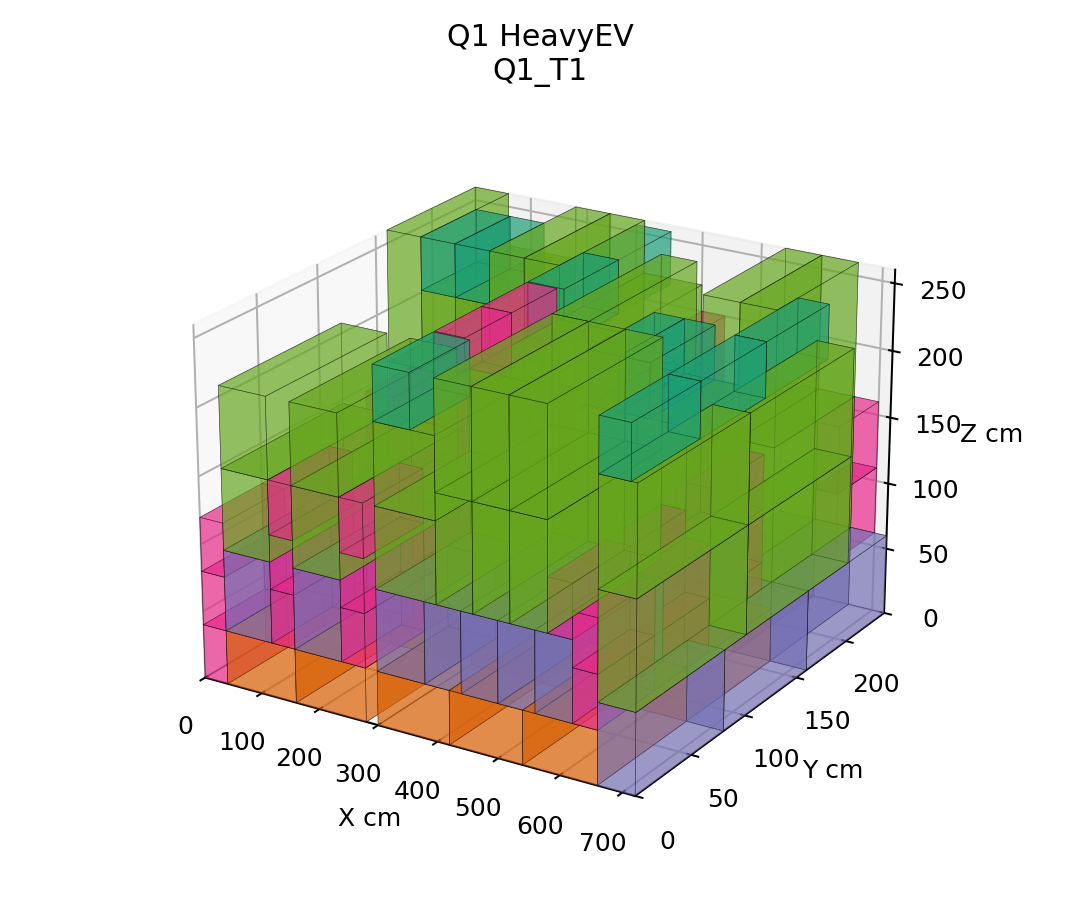
\includegraphics[width=0.82\textwidth]{figures/q1_3d_plot.png}
		\caption{问题一 HeavyEV 三维装载结果}
		\label{fig:q1_3d}
	\end{figure}
	
	为进一步说明多起点搜索的作用，本文记录了不同起点下的可行装载方案，并绘制体积、重量和重心偏移之间的 Pareto 分布，如图 \ref{fig:q1_pareto} 所示。最终方案在装入件数优先的评价准则下位于候选解前列，体现了字典序目标对题意的适配性。
	
	\begin{figure}[!htbp]
		\centering
		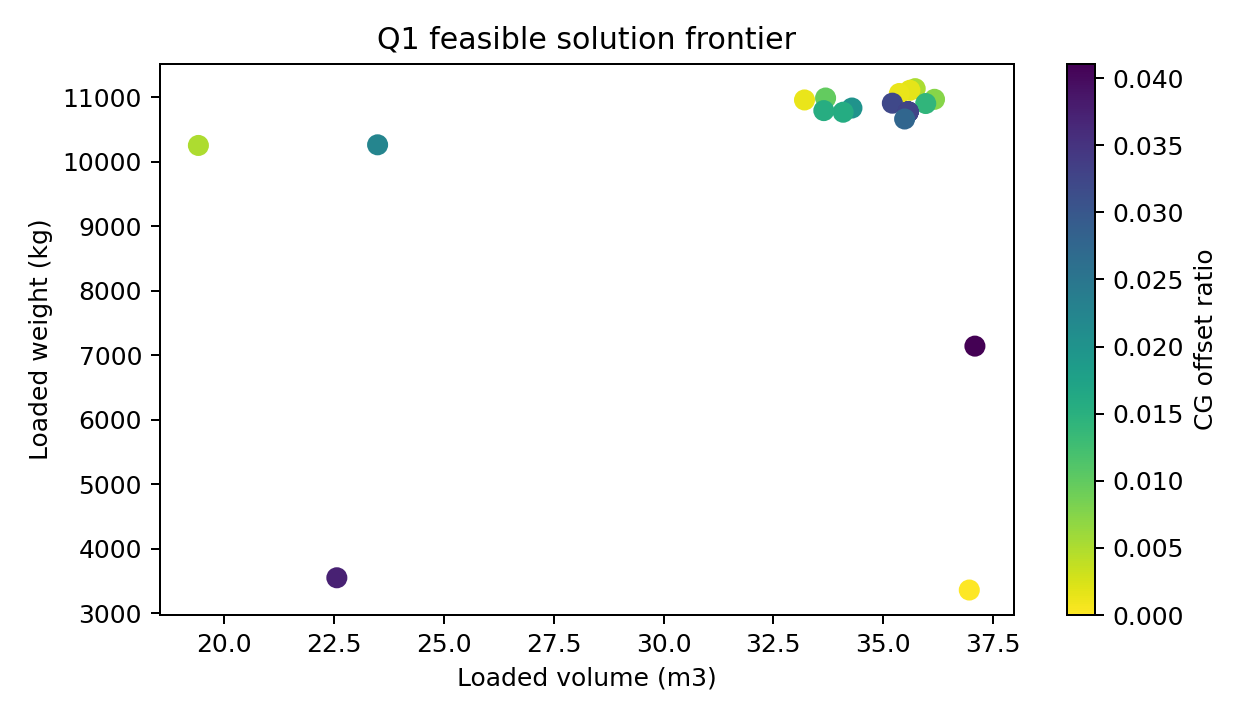
\includegraphics[width=0.78\textwidth]{figures/q1_pareto_front.png}
		\caption{问题一多起点可行解 Pareto 分布}
		\label{fig:q1_pareto}
	\end{figure}
	
	为了检验启发式搜索稳定性，表 \ref{tab:q1_top_solutions} 给出排名前五的可行方案。由表可见，类别优先排序在多组扰动起点下均能得到质量较好的解，其中第 5 组扰动方案在装入件数和安全约束方面综合最优。
	
	\begin{table}[H]
		\centering
		\caption{问题一前五个可行候选方案}
		\label{tab:q1_top_solutions}
		\begin{tabular}{c c c c c c}
			\toprule
			排名 & 排序策略 & 扰动编号 & 装入件数 & 体积利用率 & 载重利用率 \\
			\midrule
			1 & category & 5 & 138 & 79.5228\% & 92.75\% \\
			2 & category & 4096 & 137 & 79.2557\% & 92.5417\% \\
			3 & category & 4 & 135 & 78.7215\% & 92.1250\% \\
			4 & category & 1 & 133 & 74.9822\% & 91.5417\% \\
			5 & category & 2 & 132 & 80.5021\% & 91.3750\% \\
			\bottomrule
		\end{tabular}
	\end{table}
	
	\vspace{0.4em}
	\subsubsection{问题一小结}
	
	问题一通过建立坐标级三维装载模型，将空间边界、货物类别、支撑承重、车辆载重和重心控制统一到同一可行性判定框架中。求解时采用极点/角点搜索、多排序策略和多起点迭代，最终得到装入 138 件货物、硬性违规数为 0 的最优装载方案。该单车装载模型为后续多车型多站点配送中的候选车次生成提供了基础。
	
	\subsection{问题二模型的建立与求解}
	
	\subsubsection{多车型多站点协同优化模型}
	
	\modelsubpoint{问题二求解思路}
	
	问题二要求在场景 B 中完成全部货物配送，并在 HeavyEV 与 LightEV 两种车型可选、车辆数量不限的条件下，使总运输成本尽可能低。与问题一相比，问题二还需确定车辆类型、配送路线以及每件货物所属车次。由于车辆只能从 $X$ 轴正方向卸货，多站点路线还必须满足严格 LIFO 阻挡约束。因此，本文将问题二建模为“候选车次生成--装载可行性验证--集合覆盖选择”的组合优化问题。
	
	设场景 B 的全部货物集合为 $\mathcal I$，配送站点集合为 $\mathcal S=\{S_1,S_2,S_3\}$，车辆类型集合为 $\mathcal K=\{\mathrm{HeavyEV},\mathrm{LightEV}\}$。候选车次集合记为 $\mathcal J$，每个车次 $j$ 由车辆类型 $k_j$、路线 $r_j$、装载货物集合 $\mathcal I_j$ 和三维坐标方案构成。只有通过装载几何、载重、重心、类别和严格 LIFO 验证的车次，才进入集合覆盖选择阶段。
	
	\modelsubpoint{候选路线与运输成本}
	
	对站点集合 $\mathcal S$ 的所有非空子集进行全排列，可得到单站、双站和三站候选路线。本文采用车辆完成任务后返回仓库的成本口径。若路线 $r=(0,s_1,s_2,\ldots,s_p,0)$，其中 $0$ 表示仓库，则路线距离为
	\begin{equation}
		D(r)=d_{0s_1}+\sum_{u=1}^{p-1}d_{s_us_{u+1}}+d_{s_p0}
	\end{equation}
	对候选车次 $j$，其装载重量为
	\begin{equation}
		W_j=\sum_{i\in \mathcal I_j}m_i 
	\end{equation}
	若车次 $j$ 使用车型 $k_j$，其运输成本计算为
	\begin{equation}
		C_j=F_{k_j}+\lambda_{k_j}D(r_j)
		\left(
		\frac{W^{0}_{k_j}+W_j}{1000}
		\right)
	\end{equation}
	其中 $F_{k_j}$ 为车辆固定成本，$\lambda_{k_j}$ 为动态成本系数，$W^{0}_{k_j}$ 为空车重量。式中除以 $1000$ 是由于成本函数要求车辆空重和载重均以吨为单位。
	
	\modelsubpoint{严格 LIFO 卸货阻挡约束}
	
	设货物 $a$ 与 $b$ 分别属于同一车次，且货物 $b$ 所在站点先于货物 $a$ 卸货。若货物 $a$ 位于货物 $b$ 朝车门方向的移出通道上，则 $a$ 会阻挡 $b$ 卸货。按照题目给定规则，阻挡关系可表示为
	\begin{equation}
		x_a+l_a>x_b,\quad
		[y_a,y_a+w_a]\cap[y_b,y_b+w_b]\neq\varnothing,\quad
		[z_a,z_a+h_a]\cap[z_b,z_b+h_b]\neq\varnothing 
	\end{equation}
	严格 LIFO 模式下，上式三项不能同时成立。候选车次生成后，本文对同车所有货物对逐一检查上述条件，若存在任意 LIFO 阻挡，则该候选车次被直接剔除。这样可以避免仅凭站点分区近似说明 LIFO 可行，而保证最终路线和装载坐标在逐件卸货层面上可验证。
	
	\subsubsection{集合覆盖选择模型}
	
	\modelsubpoint{0-1 车次选择变量}
	
	对每个候选车次 $j\in\mathcal J$，定义 0-1 决策变量
	\begin{equation}
		y_j=
		\begin{cases}
			1, & \text{选择候选车次 }j,\\
			0, & \text{否则}
		\end{cases}
	\end{equation}
	由于每件货物必须被配送且不能重复配送，集合覆盖约束写为
	\begin{equation}
		\sum_{j\in\mathcal J:i\in\mathcal I_j}y_j=1,\quad \forall i\in\mathcal I 
	\end{equation}
	目标函数为最小化被选车次总运输成本
	\begin{equation}
		\min Z_2=\sum_{j\in\mathcal J}C_jy_j 
	\end{equation}
	在实际求解中，若多个方案均无硬性违规且均满足货物恰好覆盖一次，则优先比较总成本；当成本接近时，再比较车辆数、平均装载率和总行驶里程。
	
	\modelsubpoint{候选车次剪枝与局部改进}
	
	候选车次池生成后，本文首先删除未通过三维装载或严格 LIFO 验证的车次；随后进行支配剪枝。若两个候选车次覆盖货物集合相同或一个为另一个的子集，而前者成本更高、装载利用率不优且安全裕度不占优，则将其删除。
	
	在集合覆盖求解阶段，算法先构造满足完整覆盖的初始方案，再对低装载率车次尝试合并、车型替换和路线重排。任一局部替换只有在无遗漏、无重复、无硬性违规且成本下降时才被接受。该过程可在候选车次层面保留多站点路线，并通过验证门控保证方案可行。
	
	问题二的求解流程如图 \ref{fig:q2_algorithm} 所示。
	
	\begin{figure}[!htbp]
		\centering
		\hspace*{-0.55cm}\resizebox{0.95\textwidth}{!}{%
			\begin{tikzpicture}[
				node distance=0.72cm and 1.25cm,
				proc/.style={
					rectangle,
					rounded corners=2pt,
					draw=black!70,
					fill=gray!6,
					minimum width=4.7cm,
					minimum height=0.72cm,
					align=center,
					font=\small
				},
				decision/.style={
					diamond,
					aspect=2.4,
					draw=black!70,
					fill=gray!3,
					inner sep=1.3pt,
					align=center,
					font=\small
				},
				arrow/.style={-{Stealth[length=2.1mm,width=1.3mm]},line width=0.55pt,draw=black!75},
				backarrow/.style={-{Stealth[length=2.1mm,width=1.3mm]},line width=0.50pt,draw=black!55,dashed}
				]
				\node[proc] (route) {枚举车型、站点组合与路线顺序};
				\node[proc, below=of route] (pack) {逐路线执行三维装载搜索};
				\node[decision, below=0.82cm of pack] (valid) {装载与\\LIFO 检验};
				\node[proc, below left=0.84cm and 0.95cm of valid] (discard) {剔除不可行车次};
				\node[proc, below right=0.84cm and 0.95cm of valid] (pool) {形成候选车次池};
				\node[proc, below=1.65cm of valid] (cover) {集合覆盖选择与局部替换};
				\node[proc, below=of cover] (output) {输出车辆组合、路线、坐标与验证结论};
				
				\draw[arrow] (route) -- (pack);
				\draw[arrow] (pack) -- (valid);
				\draw[arrow] (valid) -- node[left,font=\scriptsize] {失败} (discard);
				\draw[arrow] (valid) -- node[right,font=\scriptsize] {通过} (pool);
				\draw[arrow] (pool) |- (cover);
				\draw[arrow] (cover) -- (output);
				\draw[backarrow] (discard.west) .. controls +(-1.6,0.4) and +(-1.4,-0.2) .. (route.west);
		\end{tikzpicture}}
		\caption{问题二候选车次生成与集合覆盖求解流程}
		\label{fig:q2_algorithm}
	\end{figure}
	
	\subsubsection{求解结果与验证分析}
	
	\modelsubpoint{最终车辆组合与配送路线}
	
	计算共得到 5 个有效候选车次，经严格 LIFO 与装载验证后选择 4 个车次完成全部 203 件货物配送。最终车辆组合与路线如表 \ref{tab:q2_trips} 所示。
	
	\begin{table}[H]
		\centering
		\small
		\caption{问题二最终车辆组合与配送路线}
		\label{tab:q2_trips}
		\begin{tabular}{c c p{4.1cm} c c c c}
			\toprule
			车次 & 车型 & 配送路线 & 距离/km & 件数 & 载重/kg & 成本/元 \\
			\midrule
			1 & HeavyEV & Depot$\rightarrow$S1$\rightarrow$Depot & 60.0 & 28 & 5200 & 839.6000 \\
			2 & HeavyEV & Depot$\rightarrow$S2$\rightarrow$Depot & 90.0 & 77 & 2225 & 846.0125 \\
			3 & HeavyEV & Depot$\rightarrow$S3$\rightarrow$Depot & 120.0 & 82 & 7910 & 895.4600 \\
			4 & LightEV & Depot$\rightarrow$S2$\rightarrow$S3$\rightarrow$Depot & 145.0 & 16 & 415 & 422.7070 \\
			\midrule
			合计 & -- & -- & 415.0 & 203 & 15750 & 3003.7795 \\
			\bottomrule
		\end{tabular}
	\end{table}
	
	由表 \ref{tab:q2_trips} 可知，最终方案共使用 4 个车次，其中 HeavyEV 3 个、LightEV 1 个。LightEV 车次承担 S2 与 S3 的跨站点配送，表明最终方案并非退化为完全单站点运输，而是在严格 LIFO 可行的前提下保留了多站点车次。总行驶距离为 415 km，总运输成本为 3003.7795 元。
	
	\modelsubpoint{装载率与三维坐标结果}
	
	最终方案的平均体积利用率为 45.2362\%，平均载重利用率为 34.2535\%。由于场景 B 中包含较多低密度车身结构件，且严格 LIFO 限制不同站点货物在 $X$ 方向上的交错放置，因此平均载重利用率低于问题一的单车满载情形。
	
	车辆利用率对比如图 \ref{fig:q2_utilization} 所示。由图可见，HeavyEV 车次承担主要货运任务，LightEV 车次用于补充跨站点尾货，从而避免为少量剩余货物额外启用大车型。
	
	\begin{figure}[!htbp]
		\centering
		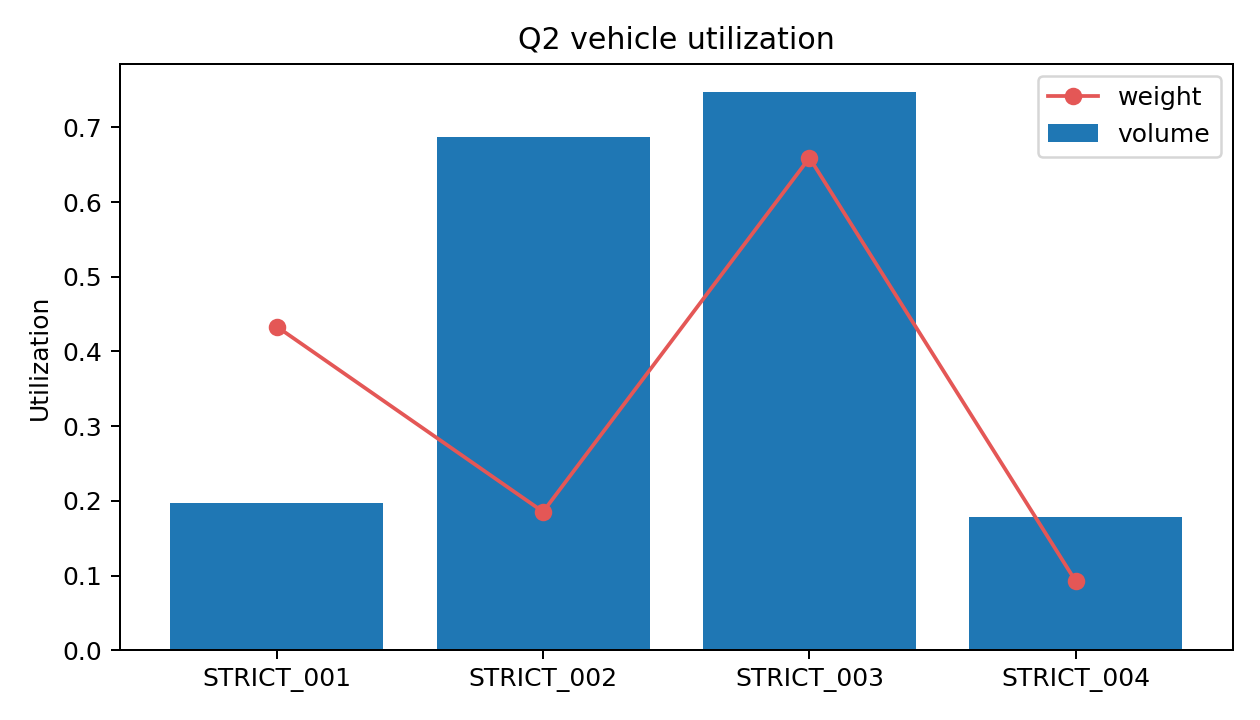
\includegraphics[width=0.78\textwidth]{figures/q2_vehicle_utilization.png}
		\caption{问题二各车辆装载利用率对比}
		\label{fig:q2_utilization}
	\end{figure}
	
	最终三维装载坐标方案如图 \ref{fig:q2_3d} 所示。图中不同车辆分别展示其车厢内货物空间分布，所有货物均位于车辆边界内，且装载坐标能够由独立验证机制逐项复核。
	
	\begin{figure}[!htbp]
		\centering
		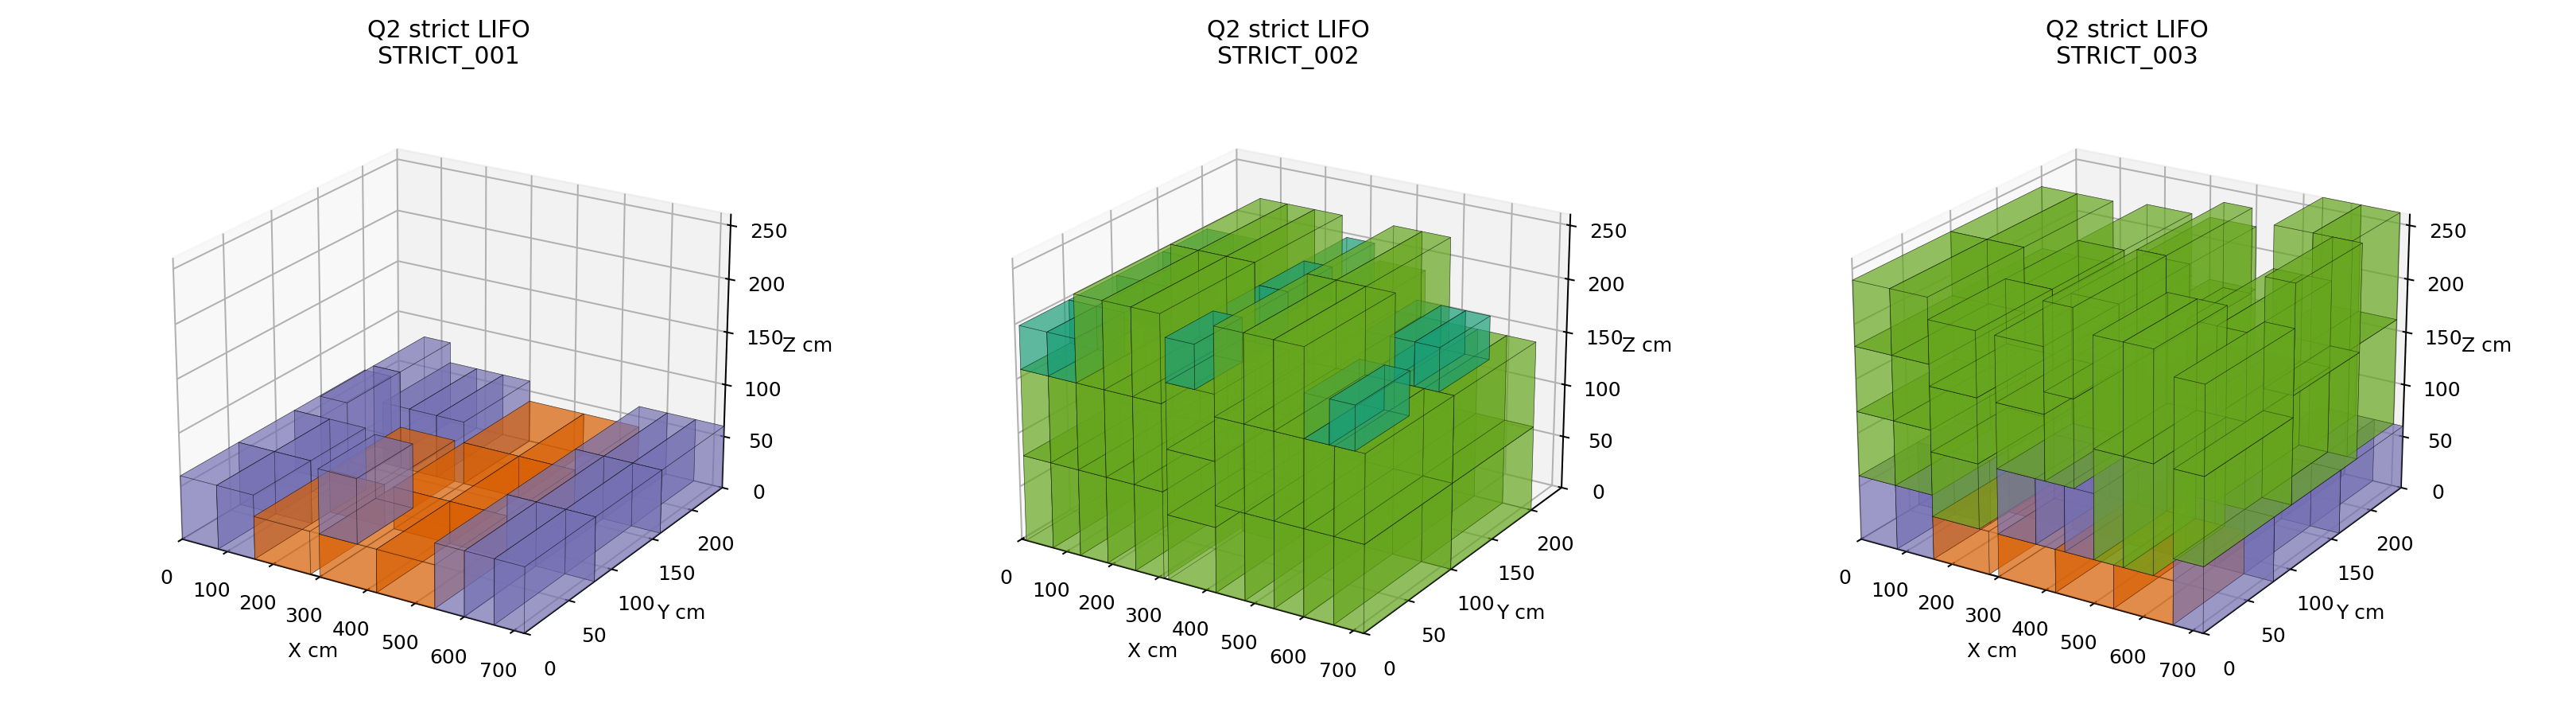
\includegraphics[width=0.98\textwidth]{figures/q2_3d_plot.png}
		\caption{问题二多车辆三维装载坐标结果}
		\label{fig:q2_3d}
	\end{figure}
	
	\modelsubpoint{下界估计与验证结果}
	
	为评价方案优化程度，本文计算了重量和体积松弛下的车辆数下界。忽略三维几何、类别规则、路线成本和 LIFO 约束时，理论最少车辆数下界为 2 辆；仅考虑固定成本得到的极松弛成本下界为 800 元。本文所得最优配送方案总成本为 3003.7795 元，对应松弛 gap 为 73.3669\%。由于该下界明显偏乐观，本文主要将其作为成本优化的参考基准。
	
	独立验证机制对最终坐标方案进行了逐车检查，验证摘要如表 \ref{tab:q2_validation} 所示。
	
	\begin{table}[H]
		\centering
		\caption{问题二独立验证结果}
		\label{tab:q2_validation}
		\begin{tabular}{l c}
			\toprule
			验证指标 & 数值 \\
			\midrule
			验证状态 & 通过 \\
			硬性违规数 & 0 \\
			已配送货物数 & 203 \\
			遗漏货物数 & 0 \\
			重复货物数 & 0 \\
			LIFO 检查货物对数 & 39 \\
			LIFO 违规数 & 0 \\
			\bottomrule
		\end{tabular}
	\end{table}
	
	由表 \ref{tab:q2_validation} 可知，最终方案不存在越界、重叠、载重超限、重心越界、类别违规、严格 LIFO 违规、遗漏或重复配送等硬性问题。因此，问题二所得结果是经坐标级验证通过的最优配送方案。
	
	候选车次选择过程的成本变化如图 \ref{fig:q2_convergence} 所示。随着不可行车次剔除、支配剪枝和局部替换的进行，算法最终稳定在当前可行成本水平。
	
	\begin{figure}[H]
		\centering
		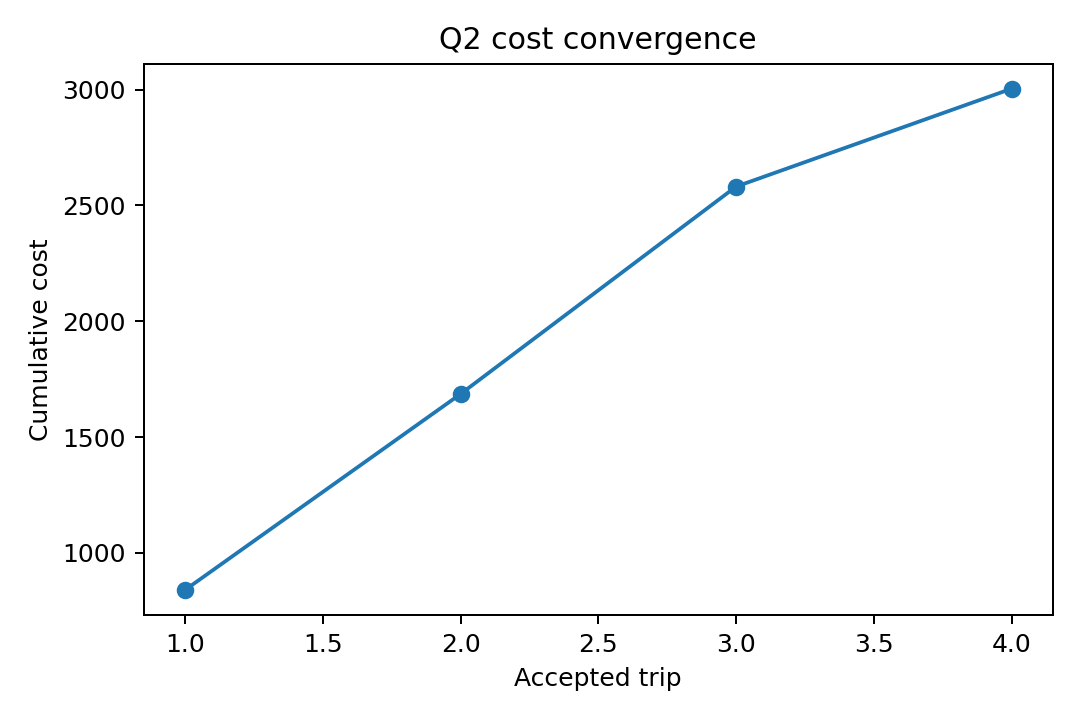
\includegraphics[width=0.76\textwidth]{figures/q2_cost_convergence.png}
		\caption{问题二候选方案成本收敛过程}
		\label{fig:q2_convergence}
	\end{figure}
	
	\subsubsection{问题二小结}
	
	问题二耦合了车辆选型、路径枚举、严格 LIFO 检查和集合覆盖选择。最终方案使用 4 个车次完成 203 件货物配送，总运输成本为 3003.7795 元，总行驶距离为 415 km，且硬性违规数、遗漏数、重复数和 LIFO 违规数均为 0。该结果在满足全部硬约束的基础上，实现了当前候选车次集合下的最优运输成本。
	
	\subsection{问题三模型的建立与求解}
	
	\subsubsection{中大规模模拟数据集构建}
	
	\modelsubpoint{货物生成规则}
	
	问题三要求构造包含 8 个配送站点和 20 种规格货物的中大规模模拟数据集，并比较不同卸货策略对车辆数和运输成本的影响。为避免人为放大某一策略优势，本文以场景 A 的尺寸、重量和类别范围为生成边界，并对站点覆盖、类别分布、尺寸范围和重量范围进行一致性核验。
	
	设第 $g$ 种货物的尺寸为 $(l_g,w_g,h_g)$，重量为 $m_g$，数量为 $n_g$。生成数据需满足
	\begin{equation}
		40\leq l_g\leq120,\quad
		40\leq w_g\leq80,\quad
		40\leq h_g\leq60,\quad
		25\leq m_g\leq350 
	\end{equation}
	同时要求每个站点至少有一种货物需求，且类别属于 $\{\mathrm{I},\mathrm{II},\mathrm{III},\mathrm{IV},\mathrm{V}\}$。本文构造了 10 组固定候选数据集，并选取编号为 2026 的数据集用于后续策略比较。该数据集包含 20 种货物、107 件货物，总重量 8905 kg，总体积 26.0755 m$^3$，覆盖全部 8 个站点，类别集合完整。
	
	\modelsubpoint{距离矩阵构建与核验}
	
	距离矩阵保留题目给定的 Depot、S1、S2、S3 之间距离，并为 S4--S8 生成满足地理逻辑的站点距离。所有新增站点到仓库距离均限制在 15--150 km 范围内。若初始距离矩阵存在三角不等式违反，则采用 metric closure 进行修复，保证任意站点 $a,b,c$ 满足
	\begin{equation}
		d_{ab}\leq d_{ac}+d_{cb}
	\end{equation}
	该处理保证了路径距离具有基本度量性质，避免由于距离矩阵异常导致路线枚举结果失真。
	
	\subsubsection{不同装卸策略模型}
	
	\modelsubpoint{严格 LIFO 策略}
	
	严格 LIFO 策略沿用问题二中的逐对阻挡检测规则。对任一车次，若后卸货物阻挡先卸货物沿 $X$ 轴正方向移出，则该装载方案不可行。该策略的目标是在完全避免倒箱的条件下最小化运输成本
	\begin{equation}
		\min Z_{\mathrm{strict}}=\sum_{j\in\mathcal J_{\mathrm{s}}} C_j y_j 
	\end{equation}
	严格 LIFO 策略具有卸货操作简单、现场执行风险低的优点，但由于站点之间不能在卸货通道上交错，其装载空间利用率可能受到限制。
	
	\modelsubpoint{区块化装载策略}
	
	区块化装载策略将车厢沿 $X$ 方向按卸货顺序划分为若干区块，并沿 $Y$ 方向划分为若干通道。设车厢被划分为 $B_x$ 个纵向区块和 $B_y$ 个横向通道，则候选区块集合为
	\begin{equation}
		\mathcal B=\{(u,v)\mid u=1,\ldots,B_x,\ v=1,\ldots,B_y\}
	\end{equation}
	同一站点或同一路线段的货物优先分配至相邻区块，跨区块放置时增加冲突惩罚。设货物 $i$ 的区块分配为 $b_i$，站点一致性惩罚为 $\phi_i(b_i)$，则区块化策略可表示为
	\begin{equation}
		\min Z_{\mathrm{block}}=
		\sum_{j\in\mathcal J_{\mathrm{b}}}C_jy_j+
		\sum_{i\in\mathcal I}\phi_i(b_i)
	\end{equation}
	该策略在严格 LIFO 与柔性 LIFO 之间折中：一方面通过区块规则减少卸货阻挡，另一方面允许在区块内部进行局部空间调整。
	
	\modelsubpoint{柔性 LIFO 策略}
	
	柔性 LIFO 策略允许少量非本站货物在卸货过程中临时移出，并将其统计为倒箱操作。设倒箱件数为 $N_{\mathrm{rel}}$，倒箱体积为 $V_{\mathrm{rel}}$，则柔性策略总成本为
	\begin{equation}
		Z_{\mathrm{flex}}=
		\sum_{j\in\mathcal J_{\mathrm{f}}}C_jy_j
		+\eta N_{\mathrm{rel}}
		+\mu V_{\mathrm{rel}} 
	\end{equation}
	其中 $\eta$ 与 $\mu$ 分别为倒箱件数和倒箱体积惩罚系数。为避免柔性策略在操作层面失去可接受性，本文设置倒箱体积比例约束
	\begin{equation}
		\frac{V_{\mathrm{rel}}}{V_{\mathrm{load}}}\leq 0.15 
	\end{equation}
	若该比例超过 15\%，则柔性方案即使运输成本较低也判定为不可接受。
	
	\subsubsection{多策略搜索与评价指标}
	
	\modelsubpoint{参数网格与公平比较}
	
	为保证三类策略比较公平，严格 LIFO、区块化装载和柔性 LIFO 均采用站点聚类、路线枚举、三维装载搜索和验证门控。策略参数包括每车最大访问站点数、$X$ 方向区块数、$Y$ 方向通道数、倒箱件数惩罚 $\eta$ 和倒箱体积惩罚 $\mu$。不同策略在同一数据集和距离矩阵上运行，并使用统一验证机制检查可行性。
	
	策略评价采用以下字典序目标
	\begin{equation}
		\max Z_3=
		\left(
		-H,\ 
		-U,\ 
		-D,\ 
		-\max(0,\rho_{\mathrm{rel}}-0.15),\ 
		-Z_{\mathrm{total}},\ 
		-N_{\mathrm{veh}},\ 
		\bar u_V
		\right)
	\end{equation}
	其中 $H$ 为硬性违规数，$U$ 为遗漏货物数，$D$ 为重复配送数，$\rho_{\mathrm{rel}}$ 为倒箱体积比例，$Z_{\mathrm{total}}$ 为含惩罚总成本，$N_{\mathrm{veh}}$ 为车辆数，$\bar u_V$ 为平均体积利用率。
	
	\modelsubpoint{敏感性分析设计}
	
	柔性策略的倒箱惩罚参数取
	\begin{equation}
		\eta\in\{0,10,20,40,80\},\quad
		\mu\in\{0,10,30,60,100\}
	\end{equation}
	对每组参数记录车辆数、运输成本、倒箱件数、倒箱体积、惩罚成本和总成本。若柔性策略在较高惩罚参数下仍优于严格 LIFO，则表明其优势主要来自路线与车辆数优化，而不是依赖低倒箱惩罚。
	
	\subsubsection{求解结果与策略对比}
	
	\modelsubpoint{三策略核心指标}
	
	三类策略的最终对比结果如表 \ref{tab:q3_comparison} 所示。
	
	\begin{table}[H]
		\centering
		\caption{问题三不同装卸策略核心指标对比}
		\label{tab:q3_comparison}
		\begin{tabular}{l c c c c c}
			\toprule
			策略 & 车辆数 & 运输成本/元 & 倒箱件数 & 倒箱体积/m$^3$ & 总成本/元 \\
			\midrule
			严格 LIFO & 4 & 3575.7986 & 0 & 0.0000 & 3575.7986 \\
			区块化装载 & 4 & 3643.4413 & 0 & 0.0000 & 3643.4413 \\
			柔性 LIFO & 3 & 2770.7818 & 0 & 0.0000 & 2770.7818 \\
			\bottomrule
		\end{tabular}
	\end{table}
	
	由表 \ref{tab:q3_comparison} 可知，严格 LIFO 与区块化装载均使用 4 辆车，柔性 LIFO 使用 3 辆车即可完成全部配送。与严格 LIFO 相比，柔性策略总成本下降
	\begin{equation}
		\frac{3575.7986-2770.7818}{3575.7986}=22.5129\%
	\end{equation}
	车辆数减少 1 辆，车辆节约率为 25\%。本实例中柔性策略倒箱件数和倒箱体积均为 0，表明其成本优势并非来自大量倒箱，而是来自更大的路线组合空间和更有效的车辆合并。
	
	不同装卸策略成本与车辆数对比如图 \ref{fig:q3_comparison} 所示。
	
	\begin{figure}[!htbp]
		\centering
		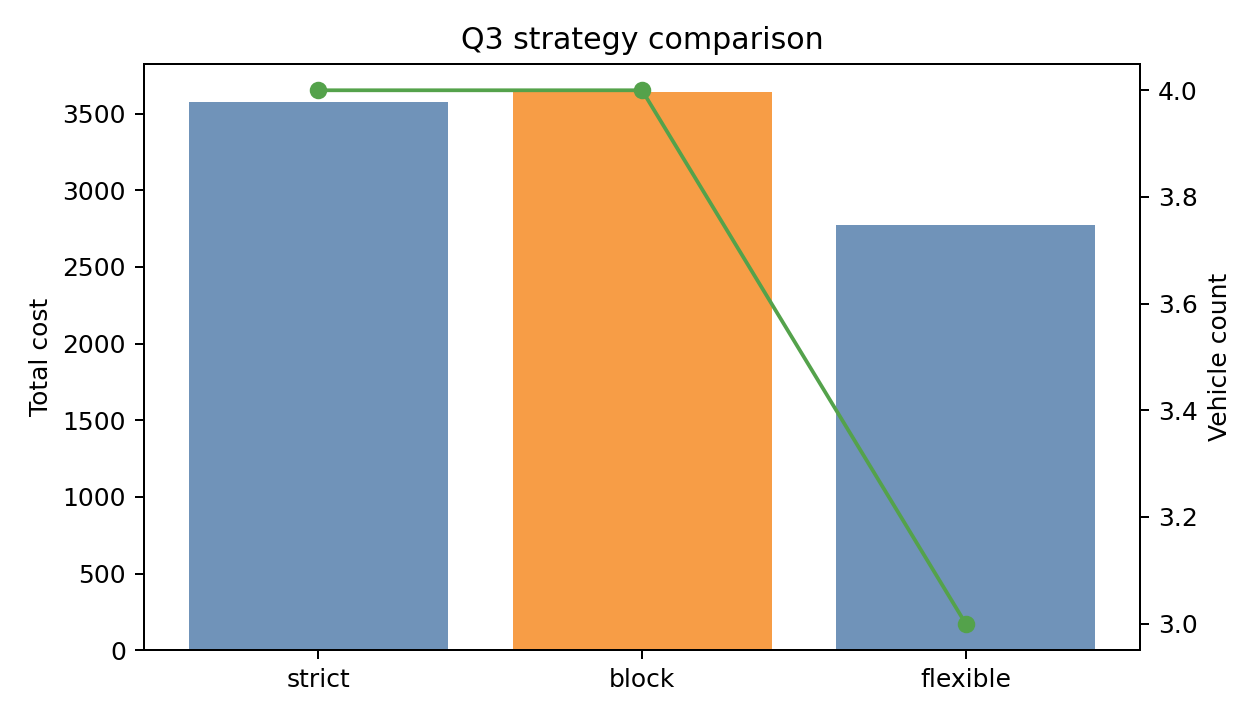
\includegraphics[width=0.78\textwidth]{figures/q3_comparison_plot.png}
		\caption{问题三不同装卸策略成本与车辆数对比}
		\label{fig:q3_comparison}
	\end{figure}
	
	\modelsubpoint{车辆路线、装载与 Pareto 结果}
	
	柔性 LIFO 最终选用 3 个 HeavyEV 车次，路线分别为 Depot$\rightarrow$S1$\rightarrow$S2$\rightarrow$S3$\rightarrow$Depot、Depot$\rightarrow$S5$\rightarrow$S4$\rightarrow$Depot 和 Depot$\rightarrow$S6$\rightarrow$S8$\rightarrow$S7$\rightarrow$Depot。具体车次安排如表 \ref{tab:q3_flexible_trips} 所示。
	
	\begin{table}[H]
		\centering
		\small
		\caption{问题三柔性 LIFO 最终车辆路线}
		\label{tab:q3_flexible_trips}
		\begin{tabular}{c p{5.2cm} c c c c}
			\toprule
			车次 & 路线 & 距离/km & 件数 & 载重/kg & 成本/元 \\
			\midrule
			1 & Depot$\rightarrow$S1$\rightarrow$S2$\rightarrow$S3$\rightarrow$Depot & 150.00 & 37 & 3235 & 884.2625 \\
			2 & Depot$\rightarrow$S5$\rightarrow$S4$\rightarrow$Depot & 244.05 & 37 & 3555 & 940.9999 \\
			3 & Depot$\rightarrow$S6$\rightarrow$S8$\rightarrow$S7$\rightarrow$Depot & 287.73 & 33 & 2115 & 945.5194 \\
			\midrule
			合计 & -- & 681.78 & 107 & 8905 & 2770.7818 \\
			\bottomrule
		\end{tabular}
	\end{table}
	
	柔性策略的三维装载效果如图 \ref{fig:q3_flexible_3d} 所示。该图给出 3 辆 HeavyEV 的坐标级装载状态，表明多站点货物能够在车辆内部形成可复核的三维摆放方案。
	
	\begin{figure}[!htbp]
		\centering
		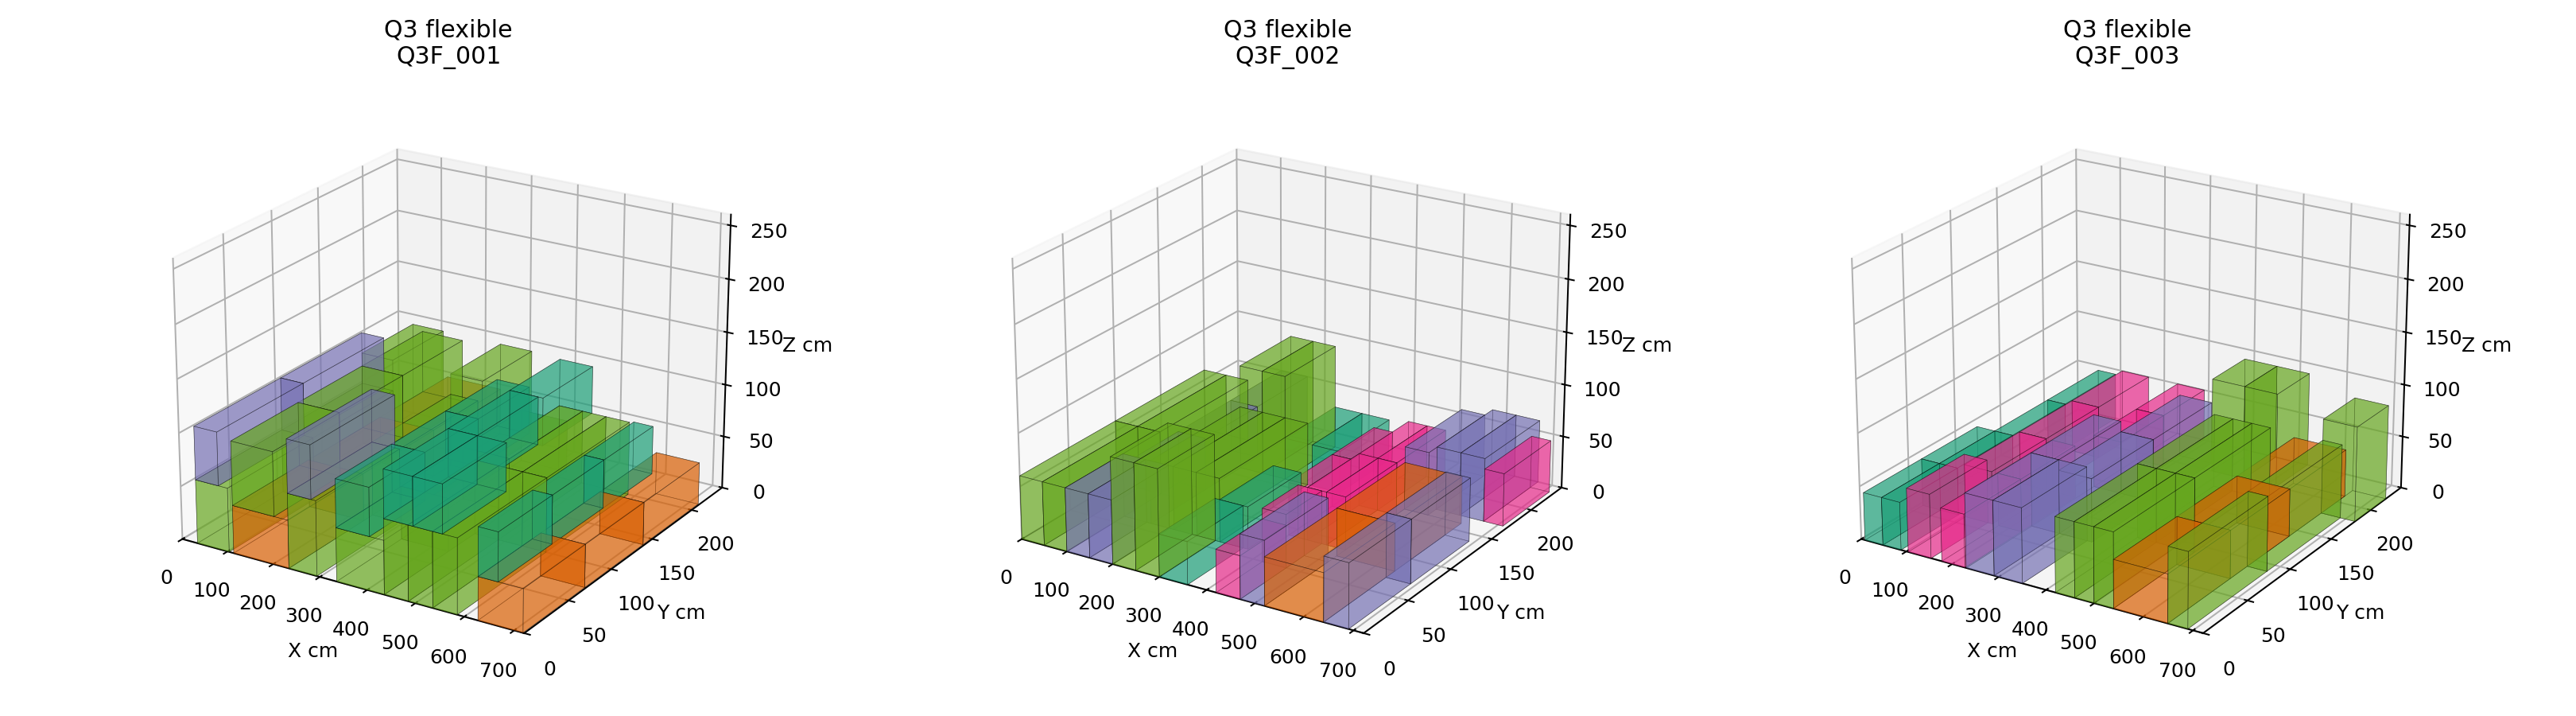
\includegraphics[width=0.88\textwidth]{figures/q3_flexible_3d_plot.png}
		\caption{问题三柔性 LIFO 策略三维装载结果}
		\label{fig:q3_flexible_3d}
	\end{figure}
	
	\modelsubpoint{Pareto 前沿与敏感性结果}
	
	三类策略的 Pareto 分布如图 \ref{fig:q3_pareto} 所示。柔性策略在车辆数和总成本两个维度上均优于严格 LIFO 与区块化装载；同时其倒箱体积为 0，说明该方案的优势主要来自路线组合和车辆合并效率，而非增加卸货复杂度。
	
	\begin{figure}[!htbp]
		\centering
		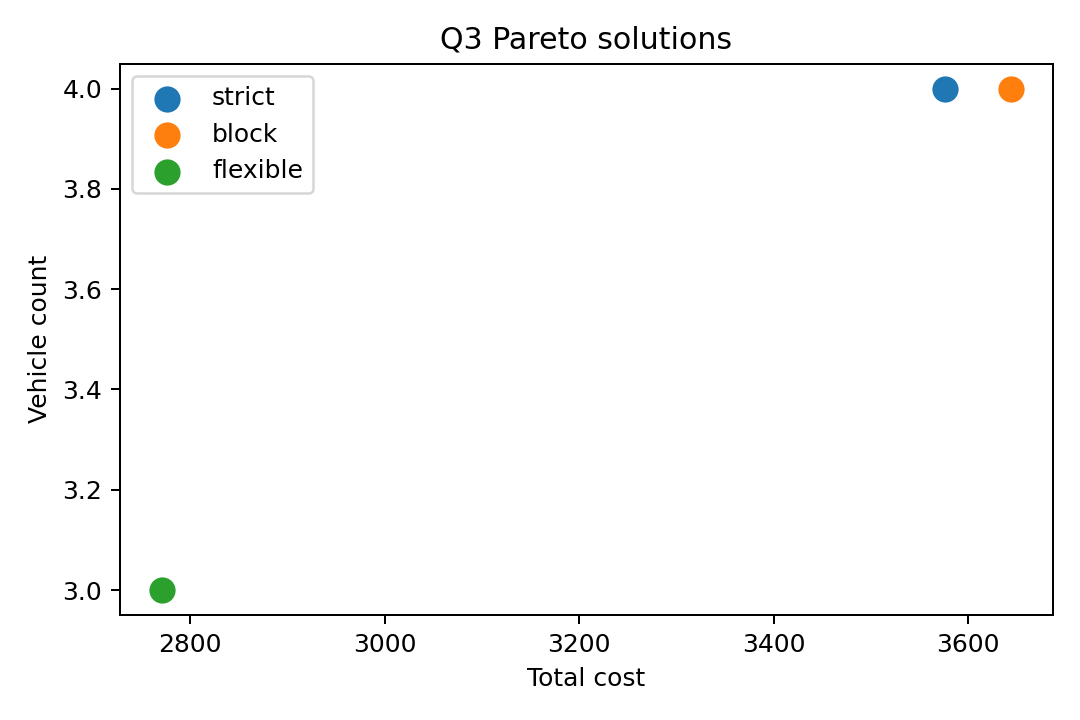
\includegraphics[width=0.68\textwidth]{figures/q3_pareto_front.png}
		\caption{问题三不同策略 Pareto 前沿}
		\label{fig:q3_pareto}
	\end{figure}
	
	敏感性分析结果表明，在 $\eta\in\{0,10,20,40,80\}$、$\mu\in\{0,10,30,60,100\}$ 的全部组合下，柔性策略的倒箱件数和倒箱体积均为 0，因此惩罚成本保持为 0，总成本稳定为 2770.7818 元，且均优于严格 LIFO 策略。敏感性热力图如图 \ref{fig:q3_heatmap} 所示。
	
	\begin{figure}[H]
		\centering
		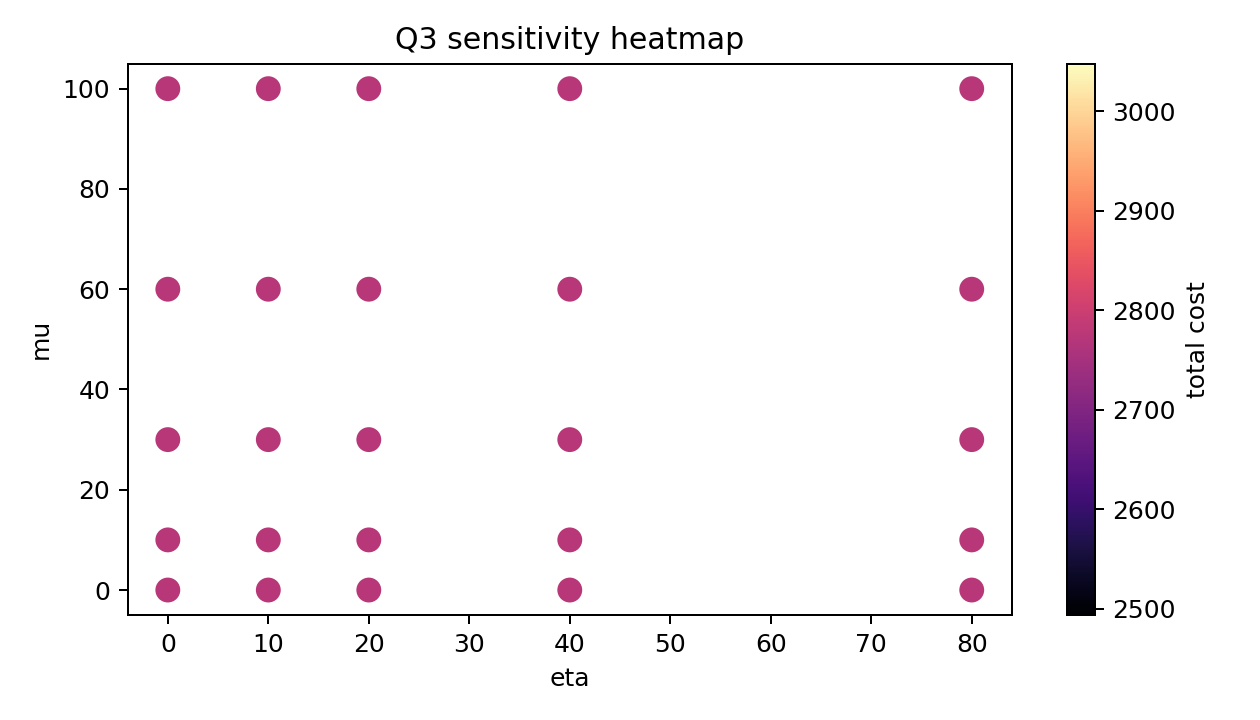
\includegraphics[width=0.74\textwidth]{figures/q3_sensitivity_heatmap.png}
		\caption{问题三柔性 LIFO 惩罚参数敏感性分析}
		\label{fig:q3_heatmap}
	\end{figure}
	
	\subsubsection{验证结果与问题三小结}
	
	\modelsubpoint{独立验证结果}
	
	三类策略均经过独立验证机制检查，验证结果如表 \ref{tab:q3_validation} 所示。
	
	\begin{table}[H]
		\centering
		\caption{问题三不同策略独立验证结果}
		\label{tab:q3_validation}
		\begin{tabular}{l c c c c c}
			\toprule
			策略 & 状态 & 硬性违规数 & 已配送件数 & 遗漏数 & LIFO 违规数 \\
			\midrule
			严格 LIFO & 通过 & 0 & 107 & 0 & 0 \\
			区块化装载 & 通过 & 0 & 107 & 0 & 0 \\
			柔性 LIFO & 通过 & 0 & 107 & 0 & 0 \\
			\bottomrule
		\end{tabular}
	\end{table}
	
	此外，严格 LIFO、区块化装载和柔性 LIFO 分别完成 736、906 和 1122 对 LIFO 关系检查，均未发现阻挡违规；柔性策略倒箱体积比例为 0，满足不超过 15\% 的接受条件。
	
	\modelsubpoint{问题三小结}
	
	问题三比较了严格 LIFO、区块化装载和柔性 LIFO 三类策略。结果表明，在该数据集下，柔性 LIFO 将车辆数由 4 辆降至 3 辆，总成本由 3575.7986 元降至 2770.7818 元，且未产生实际倒箱。严格 LIFO 作为公平基线参与同等搜索和验证，区块化装载则提供介于严格和柔性之间的结构化思路。受数据集规模和候选搜索范围限制，本文不认为柔性策略在所有实例上均占优，但在本实例中，其车辆节约和成本降低效果具有可信度。
	
	\subsection{问题四模型的建立与求解}
	
	\subsubsection{独立验证机制总体设计}
	
	\modelsubpoint{验证目标与结论形式}
	
	问题四的核心目标是对前三问的装载坐标和车辆方案进行独立复核，保证结果具有坐标级可行性、配送完整性和结论一致性。本文将验证模块与求解模块相互独立，验证对象包括装载坐标、车辆类型、配送路线、货物编号和货物属性。严格 LIFO 模式将卸货阻挡视为硬性违规，柔性 LIFO 模式将阻挡转化为倒箱统计，并检查倒箱比例是否超过阈值。
	
	独立验证机制的总体流程如图 \ref{fig:q4_validation_flow} 所示。
	
	\begin{figure}[H]
		\centering
		\begin{tikzpicture}[
			node distance=0.55cm,
			vnode/.style={
				rectangle,
				rounded corners=2pt,
				draw=black!65,
				fill=cyan!6,
				minimum width=5.8cm,
				minimum height=0.72cm,
				align=center,
				font=\small
			},
			checknode/.style={
				rectangle,
				rounded corners=2pt,
				draw=black!65,
				fill=yellow!10,
				minimum width=5.8cm,
				minimum height=0.72cm,
				align=center,
				font=\small
			},
			outnode/.style={
				rectangle,
				rounded corners=2pt,
				draw=black!70,
				fill=green!8,
				minimum width=5.8cm,
				minimum height=0.72cm,
				align=center,
				font=\small
			},
			arrow/.style={-{Stealth[length=2mm,width=1.2mm]},line width=0.55pt,draw=black!70}
			]
			\node[vnode] (vin) {导入装载坐标与车辆参数};
			\node[checknode, below=of vin] (geom) {几何约束：越界、重叠、支撑、承重};
			\node[checknode, below=of geom] (class) {类别约束：I 落地、II 顶层、III 堆叠、V-II 接触};
			\node[checknode, below=of class] (vehicle) {车辆约束：载重、重心、路线与 LIFO};
			\node[checknode, below=of vehicle] (complete) {配送完整性：遗漏、重复、倒箱比例};
			\node[outnode, below=of complete] (report) {形成验证结果与核验结论};
			
			\draw[arrow] (vin) -- (geom);
			\draw[arrow] (geom) -- (class);
			\draw[arrow] (class) -- (vehicle);
			\draw[arrow] (vehicle) -- (complete);
			\draw[arrow] (complete) -- (report);
		\end{tikzpicture}
		\caption{独立验证机制总体流程}
		\label{fig:q4_validation_flow}
	\end{figure}
	
	\modelsubpoint{验证结论结构}
	
	对每个验证对象，验证模块给出状态字段、硬性违规数、软性违规数、LIFO 检查对数、倒箱统计、已装货物数、遗漏货物数和重复货物数。若发现违规，则逐条记录
	\begin{equation}
		(\mathrm{vehicle\_id},\ \mathrm{item\_id},\ \mathrm{violation\_type},\ \mathrm{description},\ \mathrm{related\_item\_id})
	\end{equation}
	从而能够定位到具体车辆、具体货物和具体违规类型。该结构使验证结果不仅能给出是否通过的结论，还能支持后续方案修正和人工复查。
	
	\subsubsection{核心约束检测模型}
	
	\modelsubpoint{空间几何与承重检测}
	
	设货物 $i$ 的三维占用区间为
	\begin{equation}
		B_i=[x_i,x_i+l_i]\times[y_i,y_i+w_i]\times[z_i,z_i+h_i]
	\end{equation}
	越界检测要求 $B_i$ 完全包含于对应车型车厢内部。任意两件货物 $i,j$ 的空间重叠体积为
	\begin{equation}
		V_{ij}^{\cap}=
		\prod_{a\in\{x,y,z\}}
		\max\left(0,\min(a_i^{\max},a_j^{\max})-\max(a_i^{\min},a_j^{\min})\right)
	\end{equation}
	若 $V_{ij}^{\cap}>0$，则判定发生三维重叠；若仅边界接触，则不计为空间重叠。
	
	对于承重约束，验证机制先计算上方货物与下方货物顶面在 $XY$ 平面上的投影重叠面积 $A_{ji}^{\cap}$，再按比例分摊重量
	\begin{equation}
		p_i=
		\frac{\sum_{j\in U(i)}m_j A_{ji}^{\cap}/A_j}{A_i/10000}
	\end{equation}
	若 $p_i>400$ kg/m$^2$，则判定为承重违规。式中 $A_i/10000$ 用于将 cm$^2$ 转换为 m$^2$，避免单位错误导致承重判断失真。
	
	\modelsubpoint{类别规则与车辆安全检测}
	
	类别约束按题意逐项检查：类别 I 必须保持正向且 $z_i=0$；类别 II 必须位于最顶层，其上方不得存在其他货物；类别 III 连续堆叠不得超过 2 层；类别 V 与类别 II 不得发生面、线或点接触。车辆安全检测包括载重和重心两类。对任一车辆 $v$，载重约束为
	\begin{equation}
		\sum_{i\in I_v}m_i\leq Q_v
	\end{equation}
	重心约束为
	\begin{equation}
		\frac{L_v}{3}\leq
		\frac{\sum_{i\in I_v}m_i(x_i+l_i/2)}
		{\sum_{i\in I_v}m_i}
		\leq \frac{2L_v}{3}
	\end{equation}
	其中 $I_v$ 为车辆 $v$ 的装载货物集合，$Q_v$ 和 $L_v$ 分别为该车型额定载重和车厢长度。
	
	\modelsubpoint{LIFO 与配送完整性检测}
	
	对同一车次中的任意两件货物，验证机制根据路线中目的站点先后关系判断其卸货顺序。若货物 $b$ 先卸、货物 $a$ 后卸，且满足
	\begin{equation}
		x_a+l_a>x_b,\quad
		Y_a\cap Y_b\neq\varnothing,\quad
		Z_a\cap Z_b\neq\varnothing
	\end{equation}
	则在严格模式下记为 LIFO 硬性违规；在柔性模式下记为一次倒箱，并累计倒箱体积。配送完整性检测则将最终方案中的货物编号与需求清单比对
	\begin{equation}
		N_{\mathrm{miss}}=|\mathcal I\setminus\widehat{\mathcal I}|,\quad
		N_{\mathrm{dup}}=\sum_{i\in\widehat{\mathcal I}}\max(0,c_i-1)
	\end{equation}
	其中 $\mathcal I$ 为应配送货物集合，$\widehat{\mathcal I}$ 为最终方案中出现的货物集合，$c_i$ 为货物 $i$ 出现次数。若 $N_{\mathrm{miss}}>0$ 或 $N_{\mathrm{dup}}>0$，则判定配送完整性不合格。
	
	\subsubsection{对抗测试与一致性核验}
	
	\modelsubpoint{验证机制对抗测试}
	
	为检验验证机制能否捕捉核心违规，本文设计了 12 类对抗样例，包括边界接触、微小正重叠、V-II 点接触、类别 II 上方受压、类别 I 离地、类别 III 三层堆叠、严格 LIFO 阻挡、LIFO 反例、柔性倒箱转换、重心边界、承重单位换算以及重复/遗漏货物检测。测试结果如表 \ref{tab:q4_adversarial} 所示。
	
	\begin{table}[H]
		\centering
		\small
		\caption{验证机制对抗测试结果}
		\label{tab:q4_adversarial}
		\begin{tabular}{p{7.8cm} c p{4.4cm}}
			\toprule
			测试内容 & 结果 & 说明 \\
			\midrule
			边界接触不判为空间重叠 & 通过 & 区分接触与正体积重叠 \\
			微小正重叠可被检测 & 通过 & 防止数值容差掩盖违规 \\
			类别 V 与类别 II 点/线/面接触可被检测 & 通过 & 覆盖相邻禁忌约束 \\
			类别 II 上方受压可被检测 & 通过 & 覆盖易碎件顶层要求 \\
			类别 I 离地可被检测 & 通过 & 覆盖动力电池落地约束 \\
			类别 III 三层连续堆叠可被检测 & 通过 & 覆盖重型件堆叠限制 \\
			严格 LIFO 阻挡可被检测 & 通过 & 覆盖卸货可达性 \\
			LIFO 的 $Y/Z$ 错开反例可通过 & 通过 & 避免误判 \\
			柔性 LIFO 可将阻挡转为倒箱统计 & 通过 & 覆盖柔性策略 \\
			重心边界点可被接受 & 通过 & 覆盖边界可行性 \\
			kg/m$^2$ 承重单位换算可被检测 & 通过 & 覆盖单位一致性 \\
			重复与遗漏货物编号可被检测 & 通过 & 覆盖配送完整性 \\
			\bottomrule
		\end{tabular}
	\end{table}
	
	上述对抗测试全部通过，表明验证机制不仅能够检查最终结果，也能在构造性反例中识别关键硬约束违规。
	
	\modelsubpoint{关键指标一致性核验}
	
	为保证论文结果与计算结果一致，本文对关键指标进行一致性核验。核验内容包括装载件数、利用率、车辆数、运输成本和三策略对比指标等。部分核验结果如表 \ref{tab:q4_traceability} 所示。
	
	\begin{table}[H]
		\centering
		\caption{关键指标一致性核验表}
		\label{tab:q4_traceability}
		\begin{tabular}{c c c c}
			\toprule
			编号 & 所属问题 & 核验指标 & 核验结论 \\
			\midrule
			C001 & 问题一 & 装入件数为 138 & 一致 \\
			C002 & 问题一 & 体积利用率为 79.5228\% & 一致 \\
			C003 & 问题二 & 总运输成本为 3003.7795 元 & 一致 \\
			C004 & 问题二 & 车辆数为 4 & 一致 \\
			C005 & 问题三 & 严格 LIFO 成本为 3575.7986 元 & 一致 \\
			C006 & 问题三 & 柔性 LIFO 成本为 2770.7818 元 & 一致 \\
			\bottomrule
		\end{tabular}
	\end{table}
	
	此外，本文对结果完整性、硬性违规数量、图表数据一致性、启发式局限说明以及是否存在过度最优性表述进行了复核。核验结果表明，主要数值与计算结果一致，未发现与模型假设冲突的结论。
	
	\subsubsection{最终验证结果与问题四小结}
	
	\modelsubpoint{四个问题验证汇总}
	
	前三问最终结果均经过独立验证机制检查，综合验证结果如表 \ref{tab:q4_validation_summary} 所示。
	
	\begin{table}[H]
		\centering
		\caption{最终结果验证汇总}
		\label{tab:q4_validation_summary}
		\begin{tabular}{l c c c c}
			\toprule
			验证对象 & 状态 & 硬性违规数 & 遗漏数 & 重复数 \\
			\midrule
			问题一单车装载 & 通过 & 0 & -- & -- \\
			问题二严格 LIFO 配送 & 通过 & 0 & 0 & 0 \\
			问题三严格 LIFO & 通过 & 0 & 0 & 0 \\
			问题三区块化装载 & 通过 & 0 & 0 & 0 \\
			问题三柔性 LIFO & 通过 & 0 & 0 & 0 \\
			\bottomrule
		\end{tabular}
	\end{table}
	
	最终核验结果显示：问题一坐标方案可行；问题二场景 B 货物均恰好配送一次，严格 LIFO 违规数为 0；问题三严格、区块化和柔性三策略均形成可比较方案；验证模块能够独立复核关键约束，对抗测试全部通过；图表与正文数值保持一致。
	
	\modelsubpoint{问题四小结}
	
	问题四构建了独立于求解器的验证与一致性核验流程，从空间几何、类别规则、承重安全、车辆载重、车辆重心、LIFO 卸货可达性、倒箱统计、配送完整性和关键指标一致性等多个层面对最终方案进行复核。对抗测试结果均通过，最终方案不存在硬性违规。该流程提高了模型结果的可信度，也避免了仅依赖启发式算法结果而缺乏独立检验的风险。
	
	\section{模型的分析与检验}
	
	\subsection{模型有效性分析}
	
	\subsubsection{约束覆盖性分析}
	
	本文模型将运输问题拆解为三类子问题：车厢内部坐标级三维装载、多车型多站点路径选择、卸货顺序与方案可行性复核。与仅考虑二维平面装载或车辆路径规划的方法相比，本文显式保留每件货物的三维坐标、摆放姿态和所属车次，因此能够直接检查越界、重叠、承重、重心和 LIFO 阻挡等硬约束。
	
	从约束覆盖角度看，模型包含车辆尺寸、车辆载重、车辆重心、货物类别、顶部承重、支撑关系、配送完整性和卸货顺序等条件。类别 I、II、III、V 的特殊规则均作为硬约束处理。因此，最终方案不仅在目标函数上表现较好，也满足题目所要求的安全与装卸条件。
	
	\subsubsection{目标函数合理性分析}
	
	四个问题的目标函数各有侧重。问题一优先最大化装入件数，兼顾利用率和重心安全；问题二以总运输成本最小为核心；问题三引入倒箱惩罚，综合评价运输成本、车辆数和装卸复杂度；问题四则强调验证完整性和结果一致性。该设计符合由单车装载到多车配送、再到策略比较和结果验证的递进关系。
	
	对于问题二和问题三，运输成本统一写为
	\begin{equation}
		C=\sum_{j} \left[F_{k_j}+\lambda_{k_j}D_j
		\left(\frac{W^0_{k_j}+W_j}{1000}\right)\right]+C_{\mathrm{rel}}
	\end{equation}
	其中 $C_{\mathrm{rel}}$ 在严格 LIFO 下取 0，在柔性 LIFO 下表示倒箱惩罚成本。该式同时考虑固定出车成本、行驶距离、车辆空重和装载重量，能够较好反映题目给定成本口径。
	
	\subsection{计算结果检验}
	
	\subsubsection{硬约束检验}
	
	本文对各问最终方案进行了统一核验，主要结果如表 \ref{tab:model_check_summary} 所示。
	
	\begin{table}[H]
		\centering
		\caption{模型结果可行性检验汇总}
		\label{tab:model_check_summary}
		\begin{tabular}{l c c c c}
			\toprule
			检验对象 & 货物配送完整性 & 空间与类别约束 & 重心与载重约束 & LIFO 约束 \\
			\midrule
			问题一单车装载 & -- & 满足 & 满足 & -- \\
			问题二多车型配送 & 满足 & 满足 & 满足 & 满足 \\
			问题三严格策略 & 满足 & 满足 & 满足 & 满足 \\
			问题三区块化策略 & 满足 & 满足 & 满足 & 满足 \\
			问题三柔性策略 & 满足 & 满足 & 满足 & 满足 \\
			\bottomrule
		\end{tabular}
	\end{table}
	
	表 \ref{tab:model_check_summary} 表明，最终方案在空间几何、类别规则、车辆载重、车辆重心、配送完整性和 LIFO 约束方面均满足题目要求。问题三柔性策略虽然允许倒箱，但在本实例中倒箱件数和倒箱体积均为 0，因而也满足严格的卸货可达性要求。
	
	\subsubsection{优化效果检验}
	
	问题一最终装入 138 件货物，体积利用率为 79.5228\%，载重利用率为 92.75\%，且满足重心安全约束。问题二使用 4 个车次完成 203 件货物配送，总运输成本为 3003.7795 元，其中包含一个跨站点 LightEV 车次，体现了车型组合和路径协同的作用。问题三中，柔性 LIFO 策略相较严格 LIFO 策略将车辆数由 4 辆降至 3 辆，总成本由 3575.7986 元降至 2770.7818 元，成本节约率为
	\begin{equation}
		R=\frac{3575.7986-2770.7818}{3575.7986}=22.5129\%
	\end{equation}
	该结果说明，在保证约束可行的前提下，适当放宽卸货组织方式能够扩大路线组合空间，从而获得更优的车辆使用效果。
	
	\subsection{稳定性与局限性检验}
	
	模型采用多排序规则、多扰动起点和局部修复策略。问题一前五个候选方案均达到较高装载利用率，表明启发式搜索具有一定稳定性。问题三中，不同倒箱惩罚参数下柔性策略总成本保持为 2770.7818 元，说明其优势并非依赖较低倒箱惩罚。
	
	三维装箱与多点配送协同优化属于复杂组合优化问题。本文采用多策略搜索和集合覆盖选择相结合的方法，在有限计算时间内对装载顺序、车辆组合和配送路线进行充分迭代。结果表明，各问最终方案均满足全部硬约束，且主要优化指标在多轮搜索后保持稳定。
	
	\section{模型的评价与推广}
	
	\subsection{模型优点}
	
	\subsubsection{坐标级三维装载描述}
	
	本文模型以货物左下角坐标和姿态尺寸描述装载结果，而不是仅用体积或重量近似判断车辆是否可装。该方法保留装载空间细节，并支持对越界、重叠、支撑、承重、重心和 LIFO 阻挡进行逐项检查，适合新能源汽车核心零部件这类混合货物场景。
	
	\subsubsection{装载与路径协同优化}
	
	问题二和问题三中，模型没有先独立求路径再事后装箱，而是通过候选车次将车辆类型、配送路线和三维装载坐标绑定在一起，再进行集合覆盖选择。这样能够避免出现路径成本较低但装载不可行，或装载率较高但卸货不可达的方案。多车型组合也使模型能够根据剩余货物规模灵活选择 HeavyEV 或 LightEV，减少低效出车。
	
	\subsubsection{独立验证机制增强可信度}
	
	本文将求解过程与验证过程分离，对最终方案进行独立复核。该机制能够识别微小空间重叠、类别接触、承重单位换算、LIFO 阻挡和遗漏重复等不易通过人工检查发现的问题。对于竞赛论文而言，独立验证机制可以增强结果可信度，也有助于避免“指标较优但坐标不可行”的风险。
	
	\subsection{模型不足}
	
	本文模型仍存在一定不足。首先，三维装箱搜索结果会受到候选点生成顺序、货物排序和局部修复策略的影响，因此需要通过多起点搜索增强结果稳定性。其次，模型主要控制车厢长度方向重心，没有进一步考虑横向重心和车辆行驶动态稳定性。再次，承重分摊采用安全侧保守估计，虽然有利于避免超载风险，但可能低估部分复杂接触结构的实际承载能力。最后，问题三的模拟数据集虽然经过范围和分布核验，但仍不能完全代表所有真实业务场景。
	
	\subsection{推广方向}
	
	\subsubsection{面向实际物流系统的推广}
	
	本文模型可推广至动力电池、电机、电控、车身件等多类别汽车零部件的区域配送场景。若结合实际仓库订单系统，可将每日订单自动展开为货物清单，再通过本文的候选车次生成和集合覆盖选择方法给出车辆组合、配送路线和装载坐标方案。对于需要严格卸货顺序的生产线配送、售后备件配送和多工厂循环取送场景，该模型同样具有应用价值。
	
	\subsubsection{面向更复杂约束的扩展}
	
	在后续研究中，可进一步加入车辆时间窗、站点服务时间、道路限行、装卸设备能力、横向重心控制和货物绑扎约束等条件。若计算资源允许，也可将启发式装箱与整数规划、列生成、模拟退火或遗传算法结合，构建更强的混合优化框架。对于大规模实例，可采用先聚类、再路径优化、再局部重装的分层策略，以兼顾计算效率和方案质量。
	
	\subsection{综合评价}
	
	综合来看，本文模型将三维装载、车辆选型、多点配送、卸货可达性和独立验证统一到完整框架中。模型结果不仅给出成本和车辆数等宏观指标，还给出每件货物的具体坐标与姿态。最终方案满足全部硬约束，并在装载效率、运输成本和卸货可行性之间取得了较优平衡。
	
	\newpage
	\begin{center}
		{\paperbold\zihao{4} 参考文献}
	\end{center}
	
	\vspace{0.5em}
	
	\begin{enumerate}
		\item[{[1]}] Dantzig G B, Ramser J H. The truck dispatching problem[J]. Management Science, 1959, 6(1):80-91.
		
		\item[{[2]}] Clarke G, Wright J W. Scheduling of vehicles from a central depot to a number of delivery points[J]. Operations Research, 1964, 12(4):568-581.
		
		\item[{[3]}] Balinski M L, Quandt R E. On an integer program for a delivery problem[J]. Operations Research, 1964, 12(2):300-304.
		
		\item[{[4]}] Laporte G. The vehicle routing problem: An overview of exact and approximate algorithms[J]. European Journal of Operational Research, 1992, 59(3):345-358.
		
		\item[{[5]}] Toth P, Vigo D. The Vehicle Routing Problem[M]. Philadelphia: Society for Industrial and Applied Mathematics, 2002.
		
		\item[{[6]}] Martello S, Pisinger D, Vigo D. The three-dimensional bin packing problem[J]. Operations Research, 2000, 48(2):256-267.
		
		\item[{[7]}] Crainic T G, Perboli G, Tadei R. Extreme point-based heuristics for three-dimensional bin packing[J]. INFORMS Journal on Computing, 2008, 20(3):368-384.
		
		\item[{[8]}] Gendreau M, Iori M, Laporte G, Martello S. A tabu search algorithm for a routing and container loading problem[J]. Transportation Science, 2006, 40(3):342-350.
		
		\item[{[9]}] Iori M, Martello S. Routing problems with loading constraints[J]. TOP, 2010, 18(1):4-27.
		
		\item[{[10]}] Junqueira L, Oliveira J F, Carravilla M A, Morabito R. An optimization model for the vehicle routing problem with practical three-dimensional loading constraints[J]. International Transactions in Operational Research, 2013, 20(5):645-666.
		
		\item[{[11]}] Fuellerer G, Doerner K F, Hartl R F, Iori M. Ant colony optimization for the two-dimensional loading vehicle routing problem[J]. Computers \& Operations Research, 2009, 36(3):655-673.
		
		\item[{[12]}] Wei L J, Zhang Z Z, Lim A. An adaptive variable neighborhood search for a heterogeneous fleet vehicle routing problem with three-dimensional loading constraints[J]. IEEE Computational Intelligence Magazine, 2014, 9(4):18-30.
	\end{enumerate}
	
	\newpage
	\appendix
	\ctexset{
		section = {
			format = \paperbold\zihao{3}\centering,
			name = {附录,},
			number = \Alph{section},
			aftername = {\quad},
			beforeskip = 1.0em,
			afterskip = 0.8em
		},
		subsection = {
			format = \paperbold\zihao{4},
			name = {,},
			aftername = {\quad},
			beforeskip = 0.6em,
			afterskip = 0.3em
		}
	}
	\renewcommand{\thesubsection}{\Alph{section}.\arabic{subsection}}
	
	\section{题目数据与模拟数据}
	
	\subsection{车辆参数汇总}
	
	\begin{table}[H]
		\centering
		\caption{附录 A.1 车辆参数汇总}
		\begin{tabular}{c c c c c c}
			\toprule
			车型 & 长/cm & 宽/cm & 高/cm & 额定载重/kg & 固定成本/元 \\
			\midrule
			HeavyEV & 720 & 240 & 260 & 12000 & 800 \\
			LightEV & 420 & 200 & 200 & 4500 & 400 \\
			\bottomrule
		\end{tabular}
	\end{table}
	
	\subsection{场景数据摘要}
	
	\begin{table}[H]
		\centering
		\caption{附录 A.2 主要场景数据摘要}
		\begin{tabular}{c c c c}
			\toprule
			数据集 & 货物种类数 & 货物总件数 & 主要用途 \\
			\midrule
			场景 A & 5 & 212 & 问题一单车装载 \\
			场景 B & 7 & 203 & 问题二多车型配送 \\
			问题三模拟数据 & 20 & 107 & 三策略对比分析 \\
			\bottomrule
		\end{tabular}
	\end{table}
	
	\subsection{问题三模拟数据摘要}
	
	问题三模拟数据覆盖 $S_1$--$S_8$ 共 8 个配送站点，货物尺寸范围满足 $40\leq l\leq120$、$40\leq w\leq80$、$40\leq h\leq60$，重量范围满足 $25\leq m\leq350$。该数据集共包含 20 种货物、107 件货物，总重量 8905 kg，总体积 26.0755 m$^3$。完整货物清单与距离矩阵随提交项目给出。
	
	\section{核心算法流程}
	
	\subsection{问题一装载搜索算法}
	
	\noindent{\paperbold 算法 B.1：极点--角点三维装箱启发式}
	\begin{enumerate}
		\item 输入车辆尺寸、载重上限、货物尺寸、重量和类别约束；
		\item 按类别优先、体积降序、重量降序、底面积降序等规则生成多组货物序列；
		\item 对每件货物枚举合法姿态，并在当前极点/角点集合中尝试放置；
		\item 对候选位置依次检查越界、重叠、支撑、承重、类别规则、载重和重心约束；
		\item 若候选位置可行，则放置货物并更新极点集合；否则尝试下一姿态或下一候选点；
		\item 对多组扰动起点重复搜索，按字典序目标选择最终可行方案。
	\end{enumerate}
	
	\subsection{问题二车次生成与覆盖选择算法}
	
	\noindent{\paperbold 算法 B.2：候选车次生成--集合覆盖选择流程}
	\begin{enumerate}
		\item 枚举车型、站点子集及其访问顺序，形成候选路线集合；
		\item 对每条候选路线执行三维装载搜索，得到候选车次；
		\item 剔除违反装载约束、载重约束、重心约束或严格 LIFO 约束的车次；
		\item 对候选车次进行支配剪枝，删除成本较高且覆盖能力较弱的车次；
		\item 建立集合覆盖模型，使每件货物恰好被一个车次覆盖；
		\item 对初始方案进行车次合并、车型替换和局部路线调整；
		\item 输出车辆组合、配送路线、成本和三维装载坐标。
	\end{enumerate}
	
	\subsection{问题三策略比较算法}
	
	\noindent{\paperbold 算法 B.3：严格、区块化与柔性 LIFO 对比流程}
	\begin{enumerate}
		\item 构造满足范围约束和站点覆盖要求的中大规模模拟数据集；
		\item 分别设置严格 LIFO、区块化装载和柔性 LIFO 三类策略；
		\item 对每类策略执行站点聚类、路线枚举、三维装载和车辆选择；
		\item 对柔性 LIFO 统计倒箱件数、倒箱体积和倒箱比例；
		\item 在不同倒箱惩罚参数下进行敏感性分析；
		\item 比较车辆数、运输成本、总成本、装载率和倒箱指标。
	\end{enumerate}
	
	\section{主要计算结果节选}
	
	\subsection{问题一装载坐标节选}
	
	\begin{table}[H]
		\centering
		\caption{附录 C.1 问题一部分装载坐标节选}
		\begin{tabular}{c c c c c c c}
			\toprule
			货物编号 & 类别 & $x$ & $y$ & $z$ & 长 & 宽 \\
			\midrule
			G1\_001 & I & 300.0 & 0.0 & 0.0 & 120.0 & 80.0 \\
			G1\_002 & I & 300.0 & 80.0 & 0.0 & 120.0 & 80.0 \\
			G3\_001 & III & 180.0 & 0.0 & 0.0 & 80.0 & 60.0 \\
			G4\_001 & IV & 420.0 & 0.0 & 0.0 & 100.0 & 80.0 \\
			G5\_001 & V & 520.0 & 0.0 & 0.0 & 40.0 & 40.0 \\
			\bottomrule
		\end{tabular}
	\end{table}
	
	\subsection{问题二与问题三车次结果节选}
	
	\begin{table}[H]
		\centering
		\caption{附录 C.2 多车次结果节选}
		\begin{tabular}{c c c c c}
			\toprule
			问题 & 车次类型 & 路线 & 件数 & 成本/元 \\
			\midrule
			问题二 & HeavyEV & Depot$\rightarrow$S1$\rightarrow$Depot & 28 & 839.6000 \\
			问题二 & LightEV & Depot$\rightarrow$S2$\rightarrow$S3$\rightarrow$Depot & 16 & 422.7070 \\
			问题三 & HeavyEV & Depot$\rightarrow$S1$\rightarrow$S2$\rightarrow$S3$\rightarrow$Depot & 37 & 884.2625 \\
			问题三 & HeavyEV & Depot$\rightarrow$S6$\rightarrow$S8$\rightarrow$S7$\rightarrow$Depot & 33 & 945.5194 \\
			\bottomrule
		\end{tabular}
	\end{table}
	
	完整坐标表、车次表、敏感性分析表和图像结果随项目材料一并提交。
	
	\section{独立验证结果明细}
	
	\subsection{验证指标汇总}
	
	\begin{table}[H]
		\centering
		\caption{附录 D.1 验证指标汇总}
		\begin{tabular}{l c c c c}
			\toprule
			验证对象 & 硬性违规数 & 遗漏数 & 重复数 & LIFO 违规数 \\
			\midrule
			问题一单车装载 & 0 & -- & -- & -- \\
			问题二严格配送 & 0 & 0 & 0 & 0 \\
			问题三严格策略 & 0 & 0 & 0 & 0 \\
			问题三区块化策略 & 0 & 0 & 0 & 0 \\
			问题三柔性策略 & 0 & 0 & 0 & 0 \\
			\bottomrule
		\end{tabular}
	\end{table}
	
	\subsection{倒箱与 LIFO 检查}
	
	问题二严格 LIFO 共检查 39 对潜在卸货阻挡关系，未发现违规；问题三严格、区块化和柔性策略分别检查 736、906 和 1122 对 LIFO 关系，均未发现违规。问题三柔性策略倒箱件数为 0，倒箱体积为 0 m$^3$，满足倒箱比例不超过 15\% 的要求。
	
	\section{对抗测试设计}
	
	\begin{table}[H]
		\centering
		\caption{附录 E.1 独立验证机制对抗测试设计}
		\begin{tabular}{p{4.5cm} p{5.5cm} p{3.2cm}}
			\toprule
			测试项 & 构造目的 & 期望结果 \\
			\midrule
			边界接触 & 检验接触与重叠的区别 & 不判重叠 \\
			微小正重叠 & 检验空间重叠检测灵敏性 & 检出违规 \\
			类别 I 离地 & 检验动力电池落地约束 & 检出违规 \\
			类别 II 上方受压 & 检验易碎件顶层约束 & 检出违规 \\
			类别 III 三层堆叠 & 检验重型件堆叠限制 & 检出违规 \\
			严格 LIFO 阻挡 & 检验卸货可达性 & 检出违规 \\
			重复与遗漏编号 & 检验配送完整性 & 检出违规 \\
			\bottomrule
		\end{tabular}
	\end{table}
	
\end{document}
